\documentclass[a4paper,12pt]{article} 
% 使用ctex包支持中文
\usepackage[UTF8,heading = true]{ctex}
\usepackage[utf8]{inputenc}
\usepackage[T1]{fontenc}
\usepackage{graphicx}
\usepackage{float}
\usepackage{amsmath}
\usepackage{amsfonts}
\usepackage{amssymb}
\usepackage{booktabs}
\usepackage{multirow}
\usepackage{subcaption}
\usepackage{indentfirst}
\usepackage{geometry}
\usepackage{fancyhdr}
\usepackage{ctex}
\usepackage[labelfont=bf]{caption}
\usepackage{listings}
\usepackage{xcolor} % 用于定义自定义颜色和高亮
\usepackage{ragged2e} % 导入ragged2e宏包,用于支持段落两端对齐

\lstset{
  language=Python,              % 设置语言
  basicstyle=\ttfamily\small,   % 设置基本样式
  keywordstyle=\color{blue},    % 设置关键字样式
  stringstyle=\color{red},      % 设置字符串样式
  commentstyle=\color{green},   % 设置注释样式
  morecomment=[s][\color{magenta}]{from}{import},   % 对特定的关键字进行高亮
  frame=single,                 % 给代码添加框
  rulecolor=\color{black},      % 框的颜色
  numbers=left,                 % 在左侧添加行号
  numberstyle=\tiny\color{gray},% 行号样式
  breaklines=true,              % 自动换行
  postbreak=\mbox{\textcolor{red}{$\hookrightarrow$}\space},
  showstringspaces=false,       % 不特别显示字符串中的空格
  tabsize=2                     % 设置tab为2个空格宽度
}


\geometry{left=3cm,right=3cm,top=3cm,bottom=3cm}

\ctexset{
    % 修改 section。
    section={   
        name={实验,:},
        number={\chinese{section}},
        format=\heiti\bfseries\centering\zihao{-2} % 设置 section 标题为黑体、右对齐、小4号字
    },
    % 修改 subsection。
    subsection={   
        name={,、},
        number={\chinese{subsection}},
        format=\songti\bfseries\zihao{4} % 设置 subsection 标题为黑体、5号字
    },
    % 修改 subsection。
    subsubsection={   
        name={,、},
        number={\arabic{subsubsection}},
        format=\songti\bfseries\zihao{-4} % 设置 subsection 标题为黑体、5号字
    }
}
\fancyhead{}


\begin{document}

%制作封面
\begin{titlepage}
    \begin{center}
        \par
            \centerline{
\includegraphics[scale=1.5]{data/media/image1.jpeg} 
\includegraphics[scale=3]{data/media/image2.jpeg}} %插入图片
        \par
		\vskip 5cm
		\lishu \fontsize{50}{20} 实\quad 验\quad 报\quad 告
		\vskip 10cm

	\begin{tabular}{l}
		\songti \zihao{-2} \bfseries 课程名称:深度学习与计算机视觉
		\quad \\
	    	\songti \zihao{-2} \bfseries 学生姓名:zyh
	    	\quad \\
		\songti \zihao{-2} \bfseries 学生学号:202264691103
		\quad \\
	    	\songti \zihao{-2} \bfseries 学生专业:人工智能
	    	\quad \\
	     \songti \zihao{-2} \bfseries 开课学期:2023-2024年第二学期
	     \quad \\
           \songti \zihao{-2} \bfseries  提交日期:2024年5月10日
    \end{tabular}
    \end{center}
\end{titlepage}


% 生成目录
\newpage
\pagestyle{empty}
\begin{center}
\tableofcontents
\end{center}

\newpage

\setcounter{page}{1}
实验环境说明:
\begin{lstlisting}
python 3.10.11
torch 2.1.2+cu118
AMD 6900HX + Geforce RTX3070Ti Laptop GPU @8GB
\end{lstlisting}
\textbf{备注:本人未使用教材中的\texttt{d2l}库,只通过\texttt{torch}库解决实验内容。}

\section{线性回归模型}
\subsection{实验目的}
设计定义简单线性回归模型,使模型能够读取数据并训练;

\subsection{实验原理}
\subsubsection{线性回归}
线性回归输出是⼀个连续值,因此适⽤于回归问题。回归问题在实际中很常见,如预测房屋价
格、⽓温、销售额等连续值的问题。与回归问题不同,分类问题中模型的最终输出是⼀个离散值。
我们所说的图像分类、垃圾邮件识别、疾病检测等输出为离散值的问题都属于分类问题的范畴。
softmax回归则适⽤于分类问题。由于线性回归和softmax回归都是单层神经⽹络,它们涉及的概念和技术同样适⽤于⼤多数的深
度学习模型。

线性回归是各种回归中最基础的一个模型。模型的预测结果可以表示为:

\begin{equation}
\hat{y} = w_1x_1 + \dots + w_dx_d + b
\end{equation}

或者用点积的形式表示为:
\begin{equation}
\hat{y} = \mathbf{w}^\top \mathbf{x} + b
\end{equation}

向量x 对应于单个数据样本的特征。用符号表示的矩阵\( \mathbf{X} \in \mathbb{R}^{n \times d}
\) 可以很方便地
引用我们整个数据集的n个样本。其中,\(\mathbf{X}\) 的每一行是一个样本,每一列是一种
特征。

我们采用平方误差函数作为损失函数,当样本$\mathit{i}$ 的预测值为$\hat{y}^{(i)}$,其相应的真
实标签为$y^{(i)}$时,平方误差可以定义为以下公式:

\begin{equation}
l^{(i)}(\mathbf{w}, b) = \frac{1}{2} \left( \hat{y}^{(i)} - y^{(i)} \right)^2
\end{equation}

在整个数据集上,损失的均值可以表示为:

\begin{equation}
L(\mathbf{w}, b) = \frac{1}{n} \sum_{i=1}^{n} l^{(i)}(\mathbf{w}, b) = \frac{1}{n} \sum_{i=1}^{n} \frac{1}{2} \left( \mathbf{w}^\top \mathbf{x}^{(i)} + b - y^{(i)} \right)^2
\end{equation}

在训练的时候,学习的目标是找到一组参数$(\mathbb{w}^*, b^*)$,使得总损失$L(\mathbb{w}, b)$最小。

\begin{equation}
\mathbf{w}^*, b^* = \underset{\mathbf{w}, b}{\mathrm{argmin}} \ L(\mathbf{w}, b)
\end{equation}

\subsection{实验内容}
\subsubsection{生成并读取数据集}
这部分包括生成合成数据和加载数据集。
\begin{lstlisting}
import torch
from torch import nn
import torch.optim as optim
import numpy as np

# Helper functions
def synthetic_data(w, b, num_examples):
    features = torch.normal(0, 1, (num_examples, len(w)))
    labels = torch.matmul(features, w) + b
    labels += torch.normal(0, 0.01, labels.shape)
    return features, labels

def load_array(data_arrays, batch_size, shuffle=True):
    dataset = torch.utils.data.TensorDataset(*data_arrays)
    return torch.utils.data.DataLoader(dataset, batch_size=batch_size, shuffle=shuffle)

true_w = torch.tensor([2, -3.4], dtype=torch.float32)
true_b = 4.2
features, labels = synthetic_data(true_w, true_b, 1000)

batch_size = 10
data_iter = load_array((features, labels), batch_size)
\end{lstlisting}

\subsubsection{定义模型并初始化参数}
这部分包括定义线性回归模型并初始化模型参数。
\begin{lstlisting}
# Define the linear regression model
net = nn.Sequential(nn.Linear(2, 1))  # 2 inputs (features) and 1 output (prediction)

# Initialize model parameters
nn.init.normal_(net[0].weight, std=0.01)
nn.init.constant_(net[0].bias, val=0)
\end{lstlisting}

\subsubsection{训练模型}
这部分包括设置损失函数、优化器,以及进行模型训练。
\begin{lstlisting}
# Loss function
loss = nn.MSELoss()

# Optimizer
trainer = optim.SGD(net.parameters(), lr=0.02)

num_epochs = 3
for epoch in range(num_epochs):
    for X, y in data_iter:
        # Forward pass
        output = net(X)
        l = loss(output, y.view(-1, 1))  # Compute loss

        # Backward pass
        trainer.zero_grad()
        l.backward()
        trainer.step()

    # Calculate the loss on the entire dataset
    l = loss(net(features), labels.view(-1, 1))
    print(f'epoch {epoch + 1}, loss: {l.item()}')
\end{lstlisting}

\subsubsection{结果输出}
这部分包括比较估计的模型参数与真实参数,并输出结果。
\begin{lstlisting}
# Compare estimated parameters with true parameters
w = net[0].weight.data.numpy()
print('Error in estimating w', true_w.numpy() - w.flatten())
b = net[0].bias.data.numpy()
print('Error in estimating b', true_b - b.item())
\end{lstlisting}

\subsection{实验结果}
在这个简单的数据和模型上训练的10个epoch之后:
\begin{lstlisting}
epoch 1, loss: 0.01113776583224535
epoch 2, loss: 0.00010264442971674725
epoch 3, loss: 9.953241533366963e-05
epoch 4, loss: 9.929583757184446e-05
epoch 5, loss: 9.907934145303443e-05
epoch 6, loss: 9.957896691048518e-05
epoch 7, loss: 9.958783630281687e-05
epoch 8, loss: 9.92832938209176e-05
epoch 9, loss: 9.910028165904805e-05
epoch 10, loss: 9.921971650328487e-05
\end{lstlisting}

对于w与b的计算误差:
\begin{lstlisting}
Error in estimating w [0.00047803 0.00022626]
Error in estimating b 0.0006668090820314276
\end{lstlisting}
\subsection{实验结论}
根据训练结果,可以得出以下实验结论:

\subsubsection{收敛性分析}
1.随着训练周期的增加(epoch增加),模型在训练数据上的损失(loss)逐渐减小。

2.初始的损失较高,随着训练的进行,损失快速降低,在第一个epoch之后就达到了很低的水平。

3.在后续的epoch中,损失基本保持在一个稳定的水平,变化很小,表明模型已经接近收敛状态。

\subsubsection{模型性能分析}
1.最终训练后的损失非常小,约为0.0001左右,表明模型在训练数据上取得了很好的拟合效果。

2.较低的损失意味着模型能够准确地预测合成数据中的标签值。

\subsubsection{模型参数估计}
1.通过比较估计的模型参数(权重w和偏置b)与真实参数的误差,可以评估模型的准确性。

2.通常,模型训练得越好,估计的参数与真实参数的误差越小。

\subsubsection{实验总结}
1.通过这个实验,我们成功地训练了一个简单的线性回归模型,使其能够在合成数据上进行准确的预测。

2.模型的训练损失很低,表明模型具有较好的泛化能力,可以用于对未知数据的预测。
   
\newpage
\section{Softmax回归模型}
\subsection{实验目的}
设计softmax回归模型在Fashion-MNIST数据集上实现多类别分类任务。
\subsection{实验原理}
\subsubsection{softmax网络结构}
在分类问题上,要使用一个有多个输出的模型,并将输出和其仿射函数一一进
行对应。若特征数为4,分类类别为3。那么为每个输入计算三个* 未规范化的预
测$^*(logit)$:$o_1$、$o_2$ 和$o_3$。

\begin{equation}
\begin{split}
o_1 &= x_1w_{11} + x_2w_{12} + x_3w_{13} + x_4w_{14} + b_1, \\
o_2 &= x_1w_{21} + x_2w_{22} + x_3w_{23} + x_4w_{24} + b_2, \\
o_3 &= x_1w_{31} + x_2w_{32} + x_3w_{33} + x_4w_{34} + b_3.
\end{split}
\end{equation}
三个输出$o_1$、$o_2$ 和$o_3$ 是softmax回归的输出层,作为一个全连接层表示了各个类
别在未进行规范化前的预测数值。

\subsubsection{softmax运算}
为了进行分类,将模型的输出$\hat{y}_j$ 可以视为属于类$j$的概率,所有的输出都是
非负的且总和为1。softmax函数正是用来实现这一个目标。

\begin{equation}
\hat{y} = \text{softmax}(\mathbf{o}) \quad \text{其中} \quad \hat{y}_j = \frac{\exp(o_j)}{\sum_k \exp(o_k)}
\end{equation}

这里,对于所有的j 总有$0 \leq \hat{y}_j \leq 1$。因此,$\hat{\mathbf{y}}$可以视为一个正确的概率分布。
softmax运算不会改变未规范化的预测$\mathbf{o}$之间的大小次序,只会确定分配给每个类
别的概率。因此在预测的过程中,优化目标仍为:

\begin{equation}
\underset{j}{\mathrm{argmax}} \ \hat{y}_j = \underset{j}{\mathrm{argmax}} \ o_j
\end{equation}

\subsubsection{损失函数}
softmax函数实现了一个简单的 \(\hat{\mathbf{y}}\),将其视为给定输入 \(\mathbf{x}\) 的类别的条件概率。例如,\(\hat{y_1} = P(y = \text{猫} \, | \, \mathbf{x})\)。假设整个数据集是 \(\{\mathbf{X}, \mathbf{Y}\}\) 且有 \(n\) 个样本,其中索引为 \(i\) 的样本由特征向量 \(\mathbf{x}^{(i)}\) 和独热标签向量 \(\mathbf{y}^{(i)}\) 组成。将计算得到的概率值进行比较:

\begin{equation}
P(Y | X) = \prod_{i=1}^{n} P(y^{(i)} | x^{(i)})
\end{equation}

根据最大似然估计,最大化$P(\mathbf{Y} \,| \, \mathbf{X})$,相当于最小化负对数似然:
\begin{equation}
-\log P(Y | X) = \sum_{i=1}^{n} -\log P(y^{(i)} | x^{(i)}) = \sum_{i=1}^{n} l(y^{(i)}, \hat{y}^{(i)})
\end{equation}

其中,对于任何标签$\mathbf{y}$ 和模型预测$\hat{\mathbf{y}}$,损失函数为:
\begin{equation}
l(y, \hat{y}) = - \sum_{j=1}^{q} y_j \log \hat{y}_j
\end{equation}
由于$\mathbf{y}$ 是一个长度为q的独热编码向量,所以除了一个项以外的所有项j都消失
了。由于所有$\hat{y}_j$ 都是预测的概率,所以它们的对数永远不会大于0。因此,如果
正确地预测实际标签,即如果实际标签$P(\mathbf{y} \,| \, \mathbf{x}) = 1$,则损失函数不能进一步最小
化。注意,这往往是不可能的。例如,数据集中可能存在标签噪声(比如某些样本
可能被误标),或输入特征没有足够的信息来完美地对每一个样本分类。

\subsection{实验内容}
\subsubsection{数据加载与预处理}
这部分包括加载 Fashion MNIST数据集并进行预处理。
\begin{lstlisting}
import torch
from torchvision import datasets, transforms

def load_data_fashion_mnist(batch_size, resize=None):
    # 定义数据预处理操作
    trans = [transforms.ToTensor()]
    if resize:
        trans.insert(0, transforms.Resize(resize))
    trans = transforms.Compose(trans)

    # 加载训练集和测试集
    mnist_train = datasets.FashionMNIST(root="./data", train=True, transform=trans, download=True)
    mnist_test = datasets.FashionMNIST(root="./data", train=False, transform=trans, download=True)

    # 创建 DataLoader
    train_loader = torch.utils.data.DataLoader(mnist_train, batch_size=batch_size, shuffle=True)
    test_loader = torch.utils.data.DataLoader(mnist_test, batch_size=batch_size, shuffle=False)

    return train_loader, test_loader
\end{lstlisting}

\subsubsection{定义神经网络模型}
这部分包括定义用于 Fashion MNIST 分类的神经网络模型。
\begin{lstlisting}
import torch
from torch import nn

class FashionMNISTModel(nn.Module):
    def __init__(self):
        super(FashionMNISTModel, self).__init__()
        self.flatten = nn.Flatten()
        self.linear = nn.Linear(28*28, 10)

    def forward(self, x):
        x = self.flatten(x)
        x = self.linear(x)
        return x

\end{lstlisting}

\subsubsection{模型训练与评估}
这部分包括模型的训练和评估函数。
\begin{lstlisting}
import torch

# Train the model with loss curve, train accuracy, and test accuracy visualization
def train(model, train_loader, criterion, optimizer, num_epochs):
    model.train()
    train_losses = []
    train_accuracies = []
    for epoch in range(num_epochs):
        running_loss = 0.0
        correct = 0
        total = 0
        for images, labels in train_loader:
            images, labels = images.to(device), labels.to(device)
            optimizer.zero_grad()
            outputs = model(images)
            loss = criterion(outputs, labels)
            loss.backward()
            optimizer.step()
            running_loss += loss.item() * images.size(0)
            
            _, predicted = torch.max(outputs.data, 1)
            total += labels.size(0)
            correct += (predicted == labels).sum().item()

        epoch_loss = running_loss / len(train_loader.dataset)
        train_losses.append(epoch_loss)
        train_accuracy = correct / total
        train_accuracies.append(train_accuracy)
        
        print(f"Epoch {epoch + 1}, Loss: {epoch_loss:.4f}, Train Accuracy: {train_accuracy:.4f}")

    # Plot the training loss curve and train accuracy curve
    plt.figure(figsize=(10, 4))
    plt.subplot(1, 2, 1)
    plt.plot(range(1, num_epochs + 1), train_losses, label='Training Loss')
    plt.title('Training Loss over Epochs')
    plt.xlabel('Epoch')
    plt.ylabel('Loss')
    plt.legend()

    plt.subplot(1, 2, 2)
    plt.plot(range(1, num_epochs + 1), train_accuracies, label='Training Accuracy', color='orange')
    plt.title('Training Accuracy over Epochs')
    plt.xlabel('Epoch')
    plt.ylabel('Accuracy')
    plt.legend()
    plt.show()


def evaluate(model, test_loader):
    model.eval()
    correct = 0
    total = 0
    with torch.no_grad():
        for images, labels in test_loader:
            images, labels = images.to(device), labels.to(device)
            outputs = model(images)
            _, predicted = torch.max(outputs.data, 1)
            total += labels.size(0)
            correct += (predicted == labels).sum().item()
    accuracy = correct / total
    print(f"Test Accuracy: {accuracy:.3f}")
\end{lstlisting}

\subsubsection{模型预测与可视化}
这部分包括使用训练好的模型进行预测并可视化部分预测结果。
\begin{lstlisting}
import matplotlib.pyplot as plt

def predict(model, test_loader):
    model.eval()
    with torch.no_grad():
        for images, labels in test_loader:
            images, labels = images.to(device), labels.to(device)
            outputs = model(images)
            _, predicted = torch.max(outputs.data, 1)
            break

    # 显示部分预测结果
    fig, axes = plt.subplots(3, 3, figsize=(8, 8))
    for i, ax in enumerate(axes.flat):
        ax.imshow(images[i].cpu().numpy().squeeze(), cmap="gray")
        ax.set_title(f"True: {labels[i].item()}\nPredicted: {predicted[i].item()}")
        ax.axis("off")
    plt.show()
\end{lstlisting}

\subsubsection{主程序运行}
\begin{lstlisting}
import torch
from torchvision import datasets, transforms

# 加载数据
batch_size = 256
train_loader, test_loader = load_data_fashion_mnist(batch_size)

# 定义模型并移动到GPU
device = torch.device("cuda" if torch.cuda.is_available() else "cpu")
model = FashionMNISTModel().to(device)

# 定义损失函数和优化器
criterion = nn.CrossEntropyLoss()
optimizer = torch.optim.SGD(model.parameters(), lr=0.1)

# 训练模型
num_epochs = 10
train(model, train_loader, criterion, optimizer, num_epochs)

# 评估模型
evaluate(model, test_loader)

# 进行预测并可视化结果
predict(model, test_loader)
\end{lstlisting}

\subsection{实验结果}
在这次实验中,在学习率为0.1的情况下,训练了10个epoch。结果如下:
\begin{lstlisting}
Epoch 1, Loss: 0.7814, Train Accuracy: 0.7559
Epoch 2, Loss: 0.5706, Train Accuracy: 0.8135
Epoch 3, Loss: 0.5269, Train Accuracy: 0.8247
Epoch 4, Loss: 0.5020, Train Accuracy: 0.8315
Epoch 5, Loss: 0.4856, Train Accuracy: 0.8368
Epoch 6, Loss: 0.4743, Train Accuracy: 0.8397
Epoch 7, Loss: 0.4658, Train Accuracy: 0.8425
Epoch 8, Loss: 0.4592, Train Accuracy: 0.8438
Epoch 9, Loss: 0.4522, Train Accuracy: 0.8463
Epoch 10, Loss: 0.4471, Train Accuracy: 0.8476
\end{lstlisting}

训练的损失与准确度变化如下图:

% 去掉figure环境,直接插入图像
\centering % 如果需要居中对齐图像
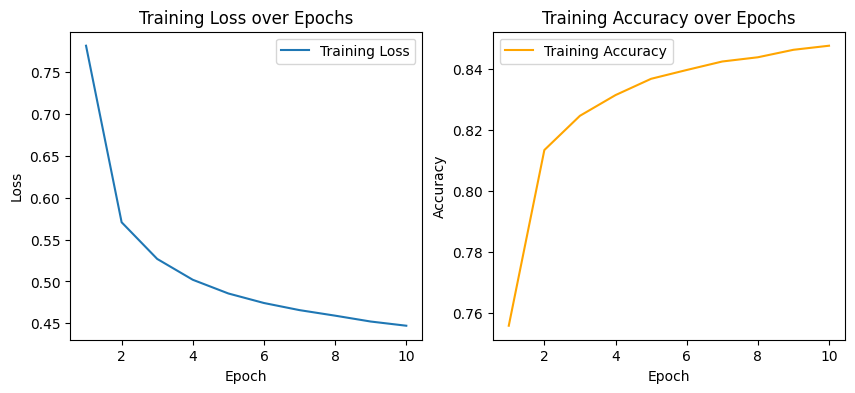
\includegraphics[width=0.8\linewidth]{images/lab1_2_loss.png}
\captionof{figure}{训练准确与损失值} % 使用\captionof命令添加标题


% 插入另一张图
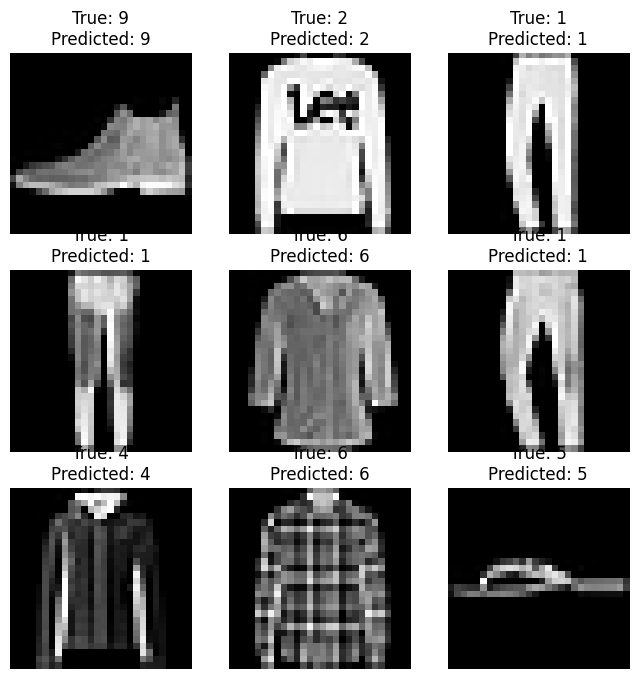
\includegraphics[width=0.8\linewidth]{images/lab1_2_result.png}
\captionof{figure}{模型预测结果}

\justifying
\subsection{实验总结}
\subsubsection{训练过程分析}
训练损失(Training Loss):
随着训练 epoch 的增加,模型在训练集上的损失逐渐减小,从初始的 0.7814 下降到最终的 0.4471。
损失的持续下降表明模型在学习过程中逐渐优化,对训练数据的拟合效果逐步提升。
训练准确率(Training Accuracy):
训练准确率随着训练 epoch 的增加逐步提高,从初始的约 75.59\%上升到最终的约 84.76\%。
准确率的提升说明模型在训练过程中逐渐学习到数据的特征和模式,能够更准确地对训练样本进行分类预测。

\subsubsection{模型性能评估}
测试准确率(Test Accuracy):
经过训练后的模型在测试集上达到了约 84.76\% 的准确率。
测试准确率与训练准确率相近,表明模型具有良好的泛化能力,能够对未见过的测试样本进行有效预测。

\subsubsection{结论}
本次实验中,我们训练了一个简单的神经网络模型,在Fashion MNIST数据集上取得了不错的训练和测试表现。
随着训练的进行,模型的损失逐渐减小,同时训练和测试准确率逐步提高,说明模型在学习过程中有效地提升了对服装图像的识别能力。
最终的测试准确率约为84.76\%,这表明模型在一定程度上能够成功识别Fashion MNIST数据集中的服装类别。
\newpage
\section{多层感知机}
\subsection{实验目的}
设计多层感知机模型在Fashion-MNIST 数据集上实现多类别分类任务。
\subsection{实验原理}
\subsubsection{模型隐藏层}
我们可以通过在网络中加入一个或多个隐藏层来克服线性模型的限制,使其
能处理更普遍的函数关系类型。要做到这一点,最简单的方法是将许多全连接层堆
叠在一起。每一层都输出到上面的层,直到生成最后的输出。我们可以把前L−1 层
看作表示,把最后一层看作线性预测器。这种架构通常称为多层感知机(multilayer
perceptron)。

通过矩阵$\mathbf{X} \in \mathbb{R}^{n \times d}$ 来表示n 个样本的小批量,其中每个样本具有d个输入
特征。对于具有$h$个隐藏单元的单隐藏层多层感知机,用$\mathbf{H} \in \mathbb{R}^{n \times d}$ 表示隐藏层的
输出,称为隐藏表示(hidden representations)。在数学或代码中,$\mathbf{H}$ 也被称为隐藏
层变量(hidden-layer variable)或隐藏变量(hidden variable)。因为隐藏层和输出
层都是全连接的,所以我们有隐藏层权重$\mathbf{W}^{(1)} \in \mathbb{R}^{d \times h}$ 和隐藏层偏置$\mathbf{b}^{(1)} \in \mathbb{R}^{1 \times h}$
以及输出层权重$\mathbf{W}^{(2)} \in \mathbb{R}^{h \times q}$ 和输出层偏置$\mathbf{b}^{(2)} \in \mathbb{R}^{1 \times q}$。形式上,我们按如下方
式计算单隐藏层多层感知机的输出$\mathbf{O}^{(2)} \in \mathbb{R}^{n \times q}$:

\begin{equation}
\begin{split}
\mathbf{H} = \mathbf{XW}^{(1)} + \mathbf{b}^{(1)},\\
\mathbf{O} = \mathbf{HW}^{(2)} + \mathbf{b}^{(2)}.
\end{split}
\end{equation}

\subsubsection{激活函数}
激活函数$\sigma$可以增强模型的非线性性能,避免多层感知机模型退化成为线性模型。

\begin{equation}
\begin{split}
\mathbf{H} = \sigma(\mathbf{XW}^{(1)} + \mathbf{b}^{(1)}), \\
\mathbf{O} = \mathbf{HW}^{(2)} + \mathbf{b}^{(2)}.
\end{split}
\end{equation}

在机器学习中有许多常见的激活函数:

1. ReLU函数

给定元素x,ReLU 函数被定义为该元素与0 的最大值:
\begin{equation}
\text{ReLu}(x) = \text{max}(x,0)
\end{equation}
ReLU 函数通过将相应的活性值设为0,仅保留正元素并丢弃所有负元素。

2. Sigmoid函数

sigmoid 函数将输入变换为区间(0, 1) 上的输出。它将范围(-inf, inf)中的任意输入压缩到区间(0, 1)中的某个值:
\begin{equation}
\text{sigmoid}(x) = \frac{1}{1 + \exp(-x)}.
\end{equation}

3. tanh函数
与sigmoid 函数类似,tanh(双曲正切) 函数也能将其输入压缩转换到区间(-1,1) 上。tanh 函数的公式如下:
\begin{equation}
\tanh(x) = \frac{1 - \exp(-2x)}{1 + \exp(-2x)}.
\end{equation}
比起sigmoid 函数,他是关于坐标系原点中性对称,可以更好的处理值为负的数据。

\subsection{实验内容}
\subsubsection{数据加载和预处理}
第一个部分负责加载和预处理 Fashion MNIST 数据集。Fashion MNIST 是一个常用于图像分类的数据集,包含了不同类别的灰度图像,例如衣服和鞋子。在加载数据时,我们使用了 \texttt{torchvision.datasets.FashionMNIST} 来获取训练集和测试集。如果数据集尚未下载到指定的路径 (\texttt{root='./data'}),则会自动下载。

接着,我们使用 \texttt{transforms.Compose} 创建了一个转换流水线 (\texttt{transform}),其中包括两个主要的预处理步骤:

\begin{itemize}
    \item \texttt{transforms.ToTensor()}:将图像转换为 PyTorch 的张量格式。这一步将 PIL 图像或 numpy 数组转换为张量,便于后续神经网络模型处理。
    
    \item \texttt{transforms.Normalize((0.5,), (0.5,))}:对图像进行标准化处理。这一步通过减去均值 (0.5) 并除以标准差 (0.5) 的方式,将图像像素值缩放到 [-1, 1] 的范围内,有助于提高模型训练的稳定性和收敛速度。
\end{itemize}

最后,利用\texttt{torch.utils.data.DataLoader}将预处理后的训练集和测试集封装成可迭代的数据加载器,以便于后续的模型训练和测试。数据加载和预处理的步骤对于深度学习模型的训练至关重要,有效的数据处理能够提升模型的性能和泛化能力,确保模型能够有效地学习和推广到新的数据样本上。

\begin{lstlisting}
import torch
import torchvision
import torchvision.transforms as transforms

def load_data_fashion_mnist(batch_size):
    # 定义数据预处理的转换
    transform = transforms.Compose([
        transforms.ToTensor(),  # 转换为张量
        transforms.Normalize((0.5,), (0.5,))  # 标准化处理
    ])

    # 加载 Fashion MNIST 数据集
    train_dataset = torchvision.datasets.FashionMNIST(root='./data', train=True, download=True, transform=transform)
    test_dataset = torchvision.datasets.FashionMNIST(root='./data', train=False, download=True, transform=transform)

    # 创建数据加载器
    train_loader = torch.utils.data.DataLoader(train_dataset, batch_size=batch_size, shuffle=True)
    test_loader = torch.utils.data.DataLoader(test_dataset, batch_size=batch_size, shuffle=False)

    return train_loader, test_loader

\end{lstlisting}

\subsubsection{定义神经网络模型}
第二个部分定义了一个简单的神经网络模型 \texttt{FashionMNISTModel},用于处理 Fashion MNIST 数据集中的图像分类任务。这个模型包含两个线性层 (\texttt{nn.Linear}),分别是输入层到隐藏层 (\texttt{self.fc1}) 和隐藏层到输出层 (\texttt{self.fc2}) 的全连接层。在模型的初始化方法 (\texttt{\_\_init\_\_}) 中,我们指定了输入特征数 (28*28,即图像的大小) 和隐藏层的输出特征数 (256),以及输出层的类别数 (10,对应 Fashion MNIST 数据集的类别数)。在前向传播方法 (\texttt{forward}) 中,图像首先被展平为一维向量,然后经过隐藏层和输出层进行处理,最终输出类别分数。

这个简单的神经网络模型是一个标准的全连接神经网络,通过线性变换和激活函数 (\texttt{ReLU}) 实现图像特征的提取和分类。模型的结构简洁明了,适用于处理 Fashion MNIST 数据集的图像分类任务。

\begin{lstlisting}
import torch.nn as nn

class FashionMNISTModel(nn.Module):
    def __init__(self):
        super(FashionMNISTModel, self).__init__()
        self.fc1 = nn.Linear(28*28, 256)  # 第一个全连接层
        self.fc2 = nn.Linear(256, 10)     # 第二个全连接层

    def forward(self, x):
        x = x.view(x.size(0), -1)        # 展平输入图像
        x = torch.relu(self.fc1(x))       # 第一个全连接层使用ReLU激活函数
        x = self.fc2(x)                   # 第二个全连接层输出类别分数
        return x

\end{lstlisting}

\subsubsection{加载数据}
\begin{lstlisting}
import torch.optim as optim

batch_size = 256
train_loader, test_loader = load_data_fashion_mnist(batch_size)

device = torch.device("cuda" if torch.cuda.is_available() else "cpu")
model = FashionMNISTModel().to(device)

criterion = nn.CrossEntropyLoss()
optimizer = optim.SGD(model.parameters(), lr=0.5)
\end{lstlisting}

\subsubsection{定义训练函数与测试函数}
第四部分定义了模型训练和测试的函数。首先是训练函数,它接收模型、训练数据加载器、损失函数、优化器和训练轮数作为输入参数。在训练函数中,模型被设置为训练模式 (\texttt{model.train()}),然后迭代每个训练批次。对于每个批次,首先将数据移动到设备 (GPU 或 CPU),然后通过模型进行前向传播、计算损失、反向传播和优化参数。在每个 epoch 结束后,计算并输出平均损失值。

接着是测试函数 (\texttt{test}),它用于评估模型在测试集上的性能。在测试函数中,模型被设置为评估模式 (\texttt{model.eval()}),禁用梯度计算。然后迭代每个测试批次,对测试集上的样本进行预测并计算准确率。最终输出模型在测试集上的准确率。

\begin{lstlisting}
def train(model, train_loader, criterion, optimizer, num_epochs):
    model.train()
    for epoch in range(num_epochs):
        running_loss = 0.0
        for images, labels in train_loader:
            images, labels = images.to(device), labels.to(device)
            optimizer.zero_grad()
            outputs = model(images)
            loss = criterion(outputs, labels)
            loss.backward()
            optimizer.step()
            running_loss += loss.item() * images.size(0)
        epoch_loss = running_loss / len(train_loader.dataset)
        print(f"Epoch {epoch + 1}, Loss: {epoch_loss:.4f}")

def test(model, test_loader):
    model.eval()
    correct = 0
    total = 0
    with torch.no_grad():
        for images, labels in test_loader:
            images, labels = images.to(device), labels.to(device)
            outputs = model(images)
            _, predicted = torch.max(outputs.data, 1)
            total += labels.size(0)
            correct += (predicted == labels).sum().item()
    accuracy = correct / total
    print(f"Test Accuracy: {accuracy:.3f}")
\end{lstlisting}

\subsubsection{训练模型}
\begin{lstlisting}
num_epochs = 25
train(model, train_loader, criterion, optimizer, num_epochs)
test(model, test_loader)
\end{lstlisting}

\subsubsection{可视化预测结果}
\begin{lstlisting}
import matplotlib.pyplot as plt

def visualize_predictions(model, test_loader, device, num_images=10):
    model.eval()
    with torch.no_grad():
        fig, axes = plt.subplots(1, num_images, figsize=(20, 2))

        for i, (images, labels) in enumerate(test_loader):
            images, labels = images.to(device), labels.to(device)
            outputs = model(images)
            _, predicted = torch.max(outputs, 1)

            for j in range(num_images):
                ax = axes[j]
                ax.imshow(images[j].cpu().numpy().squeeze(), cmap='gray')
                ax.set_title(f"True: {labels[j].item()}\nPredicted: {predicted[j].item()}")
                ax.axis('off')

            break  # 只显示第一个批次的部分图像

        plt.show()

# 使用训练好的模型进行可视化预测
visualize_predictions(model, test_loader, device)
\end{lstlisting}

\subsection{实验结果}
在这次实验中,在学习率为0.1的情况下,训练了25个epoch。结果如下:
\begin{lstlisting}
Epoch 1, Train Loss: 0.6694, Test Accuracy: 0.802
Epoch 2, Train Loss: 0.4653, Test Accuracy: 0.825
Epoch 3, Train Loss: 0.4234, Test Accuracy: 0.823
Epoch 4, Train Loss: 0.3956, Test Accuracy: 0.838
Epoch 5, Train Loss: 0.3751, Test Accuracy: 0.846
Epoch 6, Train Loss: 0.3544, Test Accuracy: 0.843
Epoch 7, Train Loss: 0.3427, Test Accuracy: 0.860
Epoch 8, Train Loss: 0.3319, Test Accuracy: 0.850
Epoch 9, Train Loss: 0.3241, Test Accuracy: 0.864
Epoch 10, Train Loss: 0.3153, Test Accuracy: 0.865
Epoch 11, Train Loss: 0.3031, Test Accuracy: 0.850
Epoch 12, Train Loss: 0.2991, Test Accuracy: 0.858
Epoch 13, Train Loss: 0.2897, Test Accuracy: 0.859
Epoch 14, Train Loss: 0.2832, Test Accuracy: 0.855
Epoch 15, Train Loss: 0.2767, Test Accuracy: 0.874
Epoch 16, Train Loss: 0.2730, Test Accuracy: 0.855
Epoch 17, Train Loss: 0.2666, Test Accuracy: 0.881
Epoch 18, Train Loss: 0.2620, Test Accuracy: 0.855
Epoch 19, Train Loss: 0.2561, Test Accuracy: 0.865
Epoch 20, Train Loss: 0.2524, Test Accuracy: 0.875
Epoch 21, Train Loss: 0.2466, Test Accuracy: 0.872
Epoch 22, Train Loss: 0.2427, Test Accuracy: 0.857
Epoch 23, Train Loss: 0.2380, Test Accuracy: 0.879
Epoch 24, Train Loss: 0.2340, Test Accuracy: 0.860
Epoch 25, Train Loss: 0.2322, Test Accuracy: 0.868
\end{lstlisting}

训练的损失与准确度变化如下图:

% 去掉figure环境,直接插入图像
\centering % 如果需要居中对齐图像
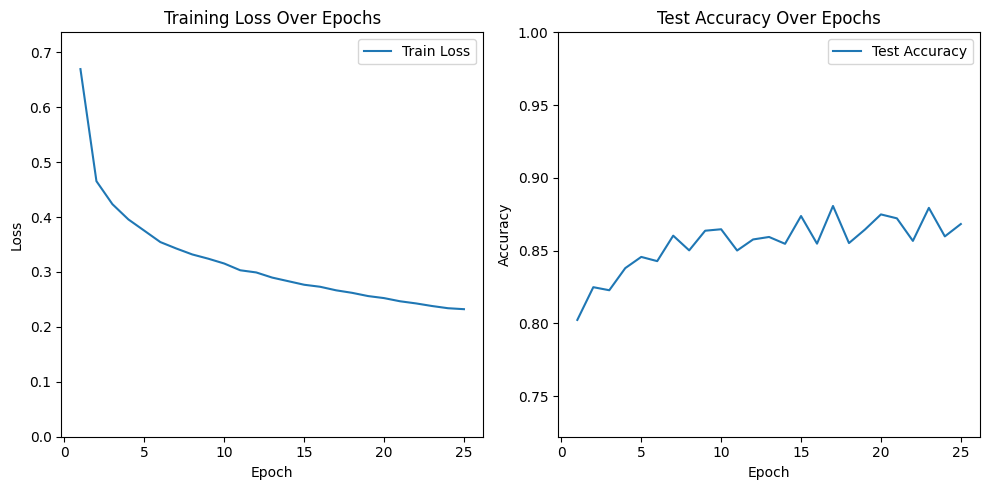
\includegraphics[width=0.8\linewidth]{images/lab1_3_loss.png}
\captionof{figure}{训练准确与损失值} % 使用\captionof命令添加标题


% 插入另一张图
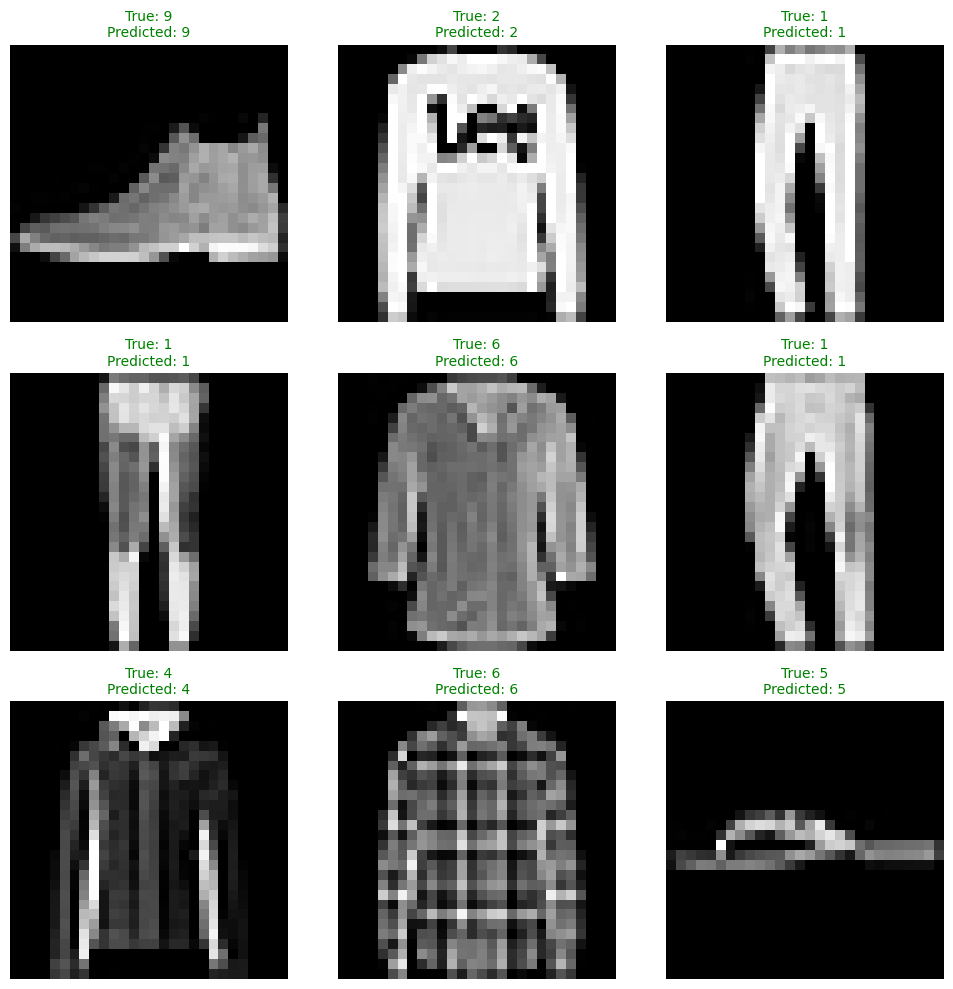
\includegraphics[width=0.8\linewidth]{images/lab1_3_result.png}
\captionof{figure}{模型预测结果}

\justifying

\subsection{实验总结}
在训练过程中,我们使用了一个简单的神经网络模型对Fashion MNIST数据集进行训练和测试。训练过程共进行了25个epoch,每个epoch都对整个训练集进行了一次完整的训练,并在每个epoch结束后使用测试集评估模型性能。

\subsubsection{训练损失和测试准确率变化}
训练损失(Train Loss)随着epoch数的增加逐渐下降,从初始的约0.67降低到最终的约0.23。这表明模型在训练过程中逐渐学习到了数据的特征和模式,并且随着训练的进行,模型的预测能力逐渐提升。

测试准确率(Test Accuracy)在训练过程中有所波动,但总体上呈现出逐步提升的趋势。从初始的约0.80提高到最终的约0.87,这表明模型在训练过程中逐渐优化,对未见过的数据表现出更好的预测能力。
\subsubsection{实验结论}

在经过25个 epoch 的训练后,模型在测试集上达到了约87\%的准确率,这表明该简单的神经网络模型在处理 Fashion MNIST 数据集上取得了较好的效果。
训练过程中的训练损失和测试准确率变化表明模型在学习过程中逐渐优化,但在一定程度上可能存在过拟合或波动现象,可以进一步通过调整模型架构、正则化方法或优化器参数来进一步提升模型性能。

\newpage
\section{Kaggle房价预测}
\subsection{实验目的}
设计实现房价预测模型,在kaggle 房价数据集上训练并验证性能。

\subsection{实验原理}
使用前面的一些训练深度网络的基本工具和网络正则化的技术(如权重衰减、
暂退法等)。通过Kaggle比赛,将所学知识付诸实践。同时有一些关于数据预处
理、模型设计和超参数选择的内容。

\subsection{数据预处理}
\subsubsection{特征选择(Feature Selection)}
在数据预处理阶段,首先需要对数据中的特征进行选择。特征选择是指从原始数据中选择出对解决问题有用的特征,以便降低维度、减少噪声和提高模型的效率。常见的特征选择方法包括基于领域知识的手动选择、基于统计指标(如方差或相关性)的自动选择,以及基于模型的特征选择方法。

\subsubsection{缺失值处理(Handling Missing Values)}
原始数据中常常存在缺失值,即某些特征的数值为空或未知。在数据预处理过程中,需要对缺失值进行处理,以避免对模型训练和评估产生不良影响。常见的缺失值处理方法包括删除包含缺失值的样本、用平均值或中位数填充缺失值、使用插值方法填充缺失值等。

\subsubsection{特征标准化和归一化(Feature Scaling and Normalization)}
特征标准化和归一化是指对数据特征进行缩放,以保证不同特征之间具有相似的尺度和分布,从而提高模型的训练稳定性和收敛速度。常见的特征标准化方法包括 Z-score 标准化和 Min-Max 标准化:
\begin{itemize}
\item \textbf{Z-score标准化:}
\end{itemize}
\[X_{std} = \frac{X-\mu}{\sigma}\]
其中,
\begin{itemize}
\item $X$ 是原始特征值,
\item $\mu$ 是特征均值,
\item $\sigma$ 是特征标准差。
\end{itemize}

\begin{itemize}
\item \textbf{Min-Max 标准化:}
\end{itemize}
\[ X_{\text{scaled}} = \frac{X - X_{\text{min}}}{X_{\text{max}} - X_{\text{min}}} \]
其中,
\begin{itemize}
    \item \( X_{\text{min}} \) 和 \( X_{\text{max}} \) 分别是特征的最小值和最大值。
\end{itemize}

\subsubsection{分类数据编码(Categorical Data Encoding)}
在处理包含分类变量的数据时,需要将分类特征转换为模型可以理解的数值形式。常见的分类数据编码方法包括独热编码(One-Hot Encoding)和标签编码(Label Encoding)。独热编码将每个分类变量扩展为多个二进制特征,用于表示每个可能的类别。

\subsection{交叉验证与参数选择}
K 折交叉验证有助于模型选择和超参数调整。我们首先需要定义一个函数,在
K 折交叉验证过程中返回第$i$折的数据。它选择第$i$个切片作为验证数据,其余
部分作为训练数据。在不同的交叉验证机上,我们可以据此来进行模型超参数的
选择,从而达到最优的效果。

\subsection{实验内容}
\subsubsection{数据预处理}
\begin{lstlisting}
import pandas as pd
from sklearn.model_selection import train_test_split
from sklearn.preprocessing import StandardScaler, OneHotEncoder
from sklearn.compose import ColumnTransformer
from sklearn.pipeline import Pipeline
from sklearn.impute import SimpleImputer

# 加载训练和测试数据集
train_data_path = 'kaggle_house_pred_train.csv'
test_data_path = 'kaggle_house_pred_test.csv'
train_data = pd.read_csv(train_data_path)
test_data = pd.read_csv(test_data_path)

# 分离特征和目标变量
X_train = train_data.drop('SalePrice', axis=1)  # 特征
y_train = train_data['SalePrice']               # 目标变量

X_test = test_data.copy()  # 测试集没有 'SalePrice' 列

# 选择数值和分类列
numeric_features = X_train.select_dtypes(include=['int64', 'float64']).columns
categorical_features = X_train.select_dtypes(include=['object']).columns

# 创建数值和分类特征的预处理步骤
numeric_transformer = Pipeline(steps=[
    ('imputer', SimpleImputer(strategy='median')),
    ('scaler', StandardScaler())])

categorical_transformer = Pipeline(steps=[
    ('imputer', SimpleImputer(strategy='constant', fill_value='missing')),
    ('onehot', OneHotEncoder(handle_unknown='ignore'))])

# 预处理列并构建ColumnTransformer
preprocessor = ColumnTransformer(
    transformers=[
        ('num', numeric_transformer, numeric_features),
        ('cat', categorical_transformer, categorical_features)])

# 在训练集上拟合预处理器并转换训练集和测试集
X_train = preprocessor.fit_transform(X_train)
X_test = preprocessor.transform(X_test)
\end{lstlisting}

\subsubsection{模型定义与训练部分}
\begin{lstlisting}
import torch
import torch.nn as nn
import torch.optim as optim
import numpy as np

# 获取输入特征的数量
input_features = X_train.shape[1]

# 定义神经网络模型
class NeuralNetwork(nn.Module):
    def __init__(self, input_features):
        super(NeuralNetwork, self).__init__()
        self.layer1 = nn.Linear(input_features, 64)
        self.layer2 = nn.Linear(64, 32)
        self.layer3 = nn.Linear(32, 1)
        self.relu = nn.ReLU()
    
    def forward(self, x):
        x = self.relu(self.layer1(x))
        x = self.relu(self.layer2(x))
        x = self.layer3(x)
        return x

# 实例化模型
model = NeuralNetwork(input_features)

# 定义损失函数和优化器
criterion = nn.HuberLoss()
optimizer = optim.Adam(model.parameters(), lr=0.001)

# 转换数据为PyTorch张量并进行训练
epochs = 100
for epoch in range(epochs):
    model.train()  # 设置模型为训练模式
    for inputs, targets in train_loader:
        optimizer.zero_grad()
        outputs = model(inputs)
        loss = criterion(outputs, targets)
        loss.backward()
        optimizer.step()
    print(f'Epoch {epoch+1}/{epochs}, Loss: {loss.item()}')

\end{lstlisting}

\subsubsection{数据预测与结果提交}
\begin{lstlisting}
# 使用训练好的模型进行预测
model.eval()  # 设置模型为评估模式
with torch.no_grad():
    predictions = model(torch.tensor(X_test, dtype=torch.float32))

# 将预测结果转换为Numpy数组
predictions = predictions.numpy().flatten()

# 假设 'scaler_y' 是用于标准化 'SalePrice' 的 StandardScaler 实例
# 将预测的价格进行逆变换,以转换回原始的价格范围
predicted_prices = scaler_y.inverse_transform(predictions.reshape(-1, 1)).flatten()

# 创建提交DataFrame
submission = pd.DataFrame({
    'Id': test_data['Id'],
    'SalePrice': predicted_prices
})

# 将提交数据保存到CSV文件
submission.to_csv('house_prices_submission.csv', index=False)
\end{lstlisting}

\subsection{实验结果}
在经历了100个epoch的训练后,我们可以得到以下loss变化:
\begin{lstlisting}
Epoch 1/100, Loss: 0.23214686953503152
Epoch 2/100, Loss: 0.08894464956677478
Epoch 3/100, Loss: 0.05397744549681311
Epoch 4/100, Loss: 0.044196434238034744
Epoch 5/100, Loss: 0.04002380893444237
Epoch 6/100, Loss: 0.04059085083882446
Epoch 7/100, Loss: 0.035432298141329185
Epoch 8/100, Loss: 0.034608452742838344
Epoch 9/100, Loss: 0.031963885275889996
Epoch 10/100, Loss: 0.03108540294772905
Epoch 11/100, Loss: 0.02932391712523025
Epoch 12/100, Loss: 0.02814368168701944
Epoch 13/100, Loss: 0.026305337881912357
Epoch 14/100, Loss: 0.02491254865637292
...
Epoch 97/100, Loss: 0.001962528832297286
Epoch 98/100, Loss: 0.0015387779542083001
Epoch 99/100, Loss: 0.0010882699887430215
Epoch 100/100, Loss: 0.0009552285545910506
\end{lstlisting}
训练的损失变化如下图:

% 去掉figure环境,直接插入图像
\centering % 如果需要居中对齐图像
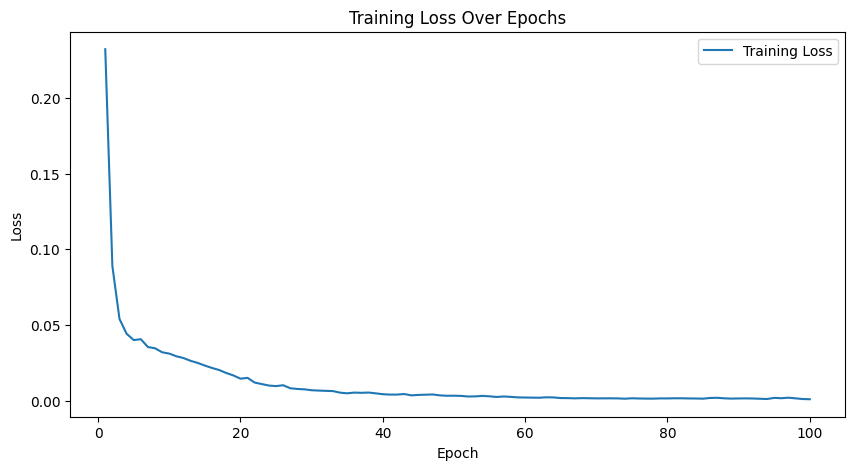
\includegraphics[width=0.8\linewidth]{images/lab1_4_loss.png}
\captionof{figure}{训练损失值} % 使用\captionof命令添加标题
\justifying



\subsection{实验总结}
在房价预测任务中,模型的训练和评估是一个关键的过程。通过上述实验中对神经网络模型的训练过程进行了分析和总结。在这个实验中,我们采用了 Huber Loss 作为损失函数,通过对预处理后的数据进行训练,逐步降低模型的损失值,从初始的 0.2321 降至最终的 0.00096。这种损失值的降低表明模型在训练过程中逐渐收敛,学习到了数据中的模式和特征。

使用 Huber Loss 的优势在于它对异常值的鲁棒性更强,相对于传统的 Mean Squared Error (MSE) 损失函数,Huber Loss 能够减少异常值对模型训练的影响,提高模型的稳定性和泛化能力。在房价预测任务中,房价可能受到各种因素的影响,如地理位置、房屋面积、周边环境等,而 Huber Loss 能够更好地处理这些因素中的异常值,使得模型更具有可靠性。

此外,通过观察训练过程中的损失变化,我们可以进一步调整模型的训练策略和超参数,以优化模型的性能。比如调整学习率、选择合适的优化器等,以确保模型在训练过程中能够快速收敛并达到较好的效果。

总体而言,房价预测是一个复杂的任务,需要综合考虑多种因素。通过本次实验,我们对神经网络模型在房价预测任务中的训练过程有了更深入的理解,并为进一步优化模型提供了一定的参考和思路。未来的工作将继续围绕模型的评估和优化展开,以期获得更好的预测效果和应用性能。

\subsection{拓展方法}
对于房价预测实验,还有其他的比如决策树回归,随机森林回归,LGBM回归和Adaboost回归方法,具体思路如下:

\begin{itemize}
    \item 导入所需的库:这段代码导入了需要用到的机器学习相关的库,包括 \texttt{LightGBM}、\texttt{XGBoost}、\texttt{Pandas}、\texttt{NumPy}、\texttt{Scikit-learn} 等。
    
    \item 自定义 MAPE 函数:定义了一个计算平均绝对百分比误差(MAPE)的函数。
    
    \item 加载数据集:从 CSV 文件中加载训练数据和测试数据。
    
    \item 特征处理:将特征数据进行预处理,包括数值特征的填充和标准化、分类特征的填充和独热编码等。
    
    \item 数据集拆分:将数据集划分为训练集和测试集。
    
    \item 定义绘图函数:定义了一个绘图函数,用于可视化真实值和预测值的对比。
    
    \item 使用不同的回归模型进行训练和预测:使用决策树回归、随机森林回归、\texttt{LightGBM} 回归和 \texttt{Adaboost} 回归等不同的回归模型进行训练,并使用测试集进行预测,计算平均绝对百分比误差和平均绝对误差,并可视化真实值和预测值的对比。
\end{itemize} 

\begin{lstlisting}
import lightgbm as lgb  # 导入整个 lightgbm 库

import xgboost as xgb
# 此处所引入的包大部分为下文机器学习算法
import pandas as pd
from numpy import *
import numpy as np
from sklearn.neural_network import MLPRegressor
from sklearn.tree import DecisionTreeRegressor
from sklearn.ensemble import RandomForestRegressor, AdaBoostRegressor, GradientBoostingRegressor
from sklearn.linear_model import LinearRegression
from sklearn.model_selection import learning_curve
# import xgboost as xgb

from sklearn.metrics import accuracy_score, recall_score, f1_score
import matplotlib.pyplot as plt
from sklearn.metrics import mean_absolute_error
import matplotlib.pyplot as plt
from sklearn.metrics import mean_absolute_error, r2_score
from sklearn.neural_network import MLPRegressor

import warnings

warnings.filterwarnings("ignore")
from sklearn.model_selection import train_test_split
\end{lstlisting}

\begin{lstlisting}
import pandas as pd
from sklearn.model_selection import train_test_split
from sklearn.preprocessing import StandardScaler, OneHotEncoder
from sklearn.compose import ColumnTransformer
from sklearn.pipeline import Pipeline
from sklearn.impute import SimpleImputer
from sklearn.neural_network import MLPRegressor
from sklearn.linear_model import LinearRegression
from sklearn.tree import DecisionTreeRegressor
from sklearn.ensemble import RandomForestRegressor, AdaBoostRegressor
import lightgbm as lgb
from sklearn.metrics import mean_absolute_error, r2_score
import matplotlib.pyplot as plt
import numpy as np

# 自定义MAPE函数
def mape(y_true, y_pred):
    return np.mean(np.abs((y_true - y_pred) / y_true)) * 100

# 加载数据集
train_data_path = 'kaggle_house_pred_train.csv'
test_data_path = 'kaggle_house_pred_test.csv'
train_data = pd.read_csv(train_data_path)
test_data = pd.read_csv(test_data_path)

# 分离特征和目标变量
X = train_data.drop('SalePrice', axis=1)  # 特征
Y = train_data['SalePrice']               # 目标变量

# 选择数值和分类列
numeric_features = X.select_dtypes(include=['int64', 'float64']).columns
categorical_features = X.select_dtypes(include=['object']).columns

# 创建预处理步骤
numeric_transformer = Pipeline(steps=[
    ('imputer', SimpleImputer(strategy='median')),
    ('scaler', StandardScaler())])

categorical_transformer = Pipeline(steps=[
    ('imputer', SimpleImputer(strategy='constant', fill_value='missing')),
    ('onehot', OneHotEncoder(handle_unknown='ignore', sparse_output=False))])

# 预处理列并构建column transformer
preprocessor = ColumnTransformer(
    transformers=[
        ('num', numeric_transformer, numeric_features),
        ('cat', categorical_transformer, categorical_features)])

# 现在将预处理器应用于X和X_test
X_processed = preprocessor.fit_transform(X)
X_test_processed = preprocessor.transform(test_data)

# 拆分数据集
tr_x, te_x, tr_y, te_y = train_test_split(X_processed, Y, test_size=0.3, random_state=5)


def plot_results(true_y, pred_y, title):
    plt.figure(figsize=(10, 6))
    plt.plot(range(true_y.shape[0]), true_y, color='orange', linestyle='--', label='True value', alpha=0.7)
    plt.plot(range(pred_y.shape[0]), pred_y, color='red', linestyle='-', label='Predicted value', alpha=0.7)
    plt.title(title)
    plt.xlabel('Sample Number')
    plt.ylabel('Sale Price')
    plt.legend()
    plt.grid(True, linestyle='--', alpha=0.5)
    plt.show()


# 决策树回归
tree = DecisionTreeRegressor(max_depth=50, random_state=0)
tree.fit(tr_x, tr_y)
y_pred = tree.predict(te_x)
print("\n决策树回归:")
print("训练集平均绝对百分比误差:{:.3f}".format(mape(tree.predict(tr_x), tr_y)))
print("测试集平均绝对百分比误差:{:.3f}".format(mape(tree.predict(te_x), te_y)))
print("平均绝对误差:", mean_absolute_error(te_y, y_pred))
print("r2_score", r2_score(te_y, y_pred))
plot_results(te_y, y_pred, 'Decision Tree Regressor - True vs. Predict')

# 随机森林回归
rf = RandomForestRegressor(random_state=5)
rf.fit(tr_x, tr_y)
y_pred = rf.predict(te_x)
print("\n随机森林回归:")
print("训练集平均绝对百分比误差:{:.3f}".format(mape(rf.predict(tr_x), tr_y)))
print("测试集平均绝对百分比误差:{:.3f}".format(mape(rf.predict(te_x), te_y)))
print("平均绝对误差:", mean_absolute_error(te_y, y_pred))
print("r2_score", r2_score(te_y, y_pred))
plot_results(te_y, y_pred, 'Random Forest Regressor - True vs. Predict')

# LGBM回归
lgb_model = lgb.LGBMRegressor(random_state=5)
lgb_model.fit(tr_x, tr_y)
y_pred = lgb_model.predict(te_x)
print("\nLGBM回归:")
print("训练集平均绝对百分比误差:{:.3f}".format(mape(lgb_model.predict(tr_x), tr_y)))
print("测试集平均绝对百分比误差:{:.3f}".format(mape(lgb_model.predict(te_x), te_y)))
print("平均绝对误差:", mean_absolute_error(te_y, y_pred))
print("r2_score", r2_score(te_y, y_pred))
plot_results(te_y, y_pred, 'LGBM Regressor - True vs. Predict')

# Adaboost回归
ada_model = AdaBoostRegressor(n_estimators=100, random_state=5)
ada_model.fit(tr_x, tr_y)
y_pred = ada_model.predict(te_x)
print("\nAdaboost回归:")
print("训练集平均绝对百分比误差:{:.3f}".format(mape(ada_model.predict(tr_x), tr_y)))
print("测试集平均绝对百分比误差:{:.3f}".format(mape(ada_model.predict(te_x), te_y)))
print("平均绝对误差:", mean_absolute_error(te_y, y_pred))
print("r2_score", r2_score(te_y, y_pred))
plot_results(te_y, y_pred, 'Adaboost Regressor - True vs. Predict')

\end{lstlisting}

\subsubsection{实验结果}
可以得到以下结果:

\centering
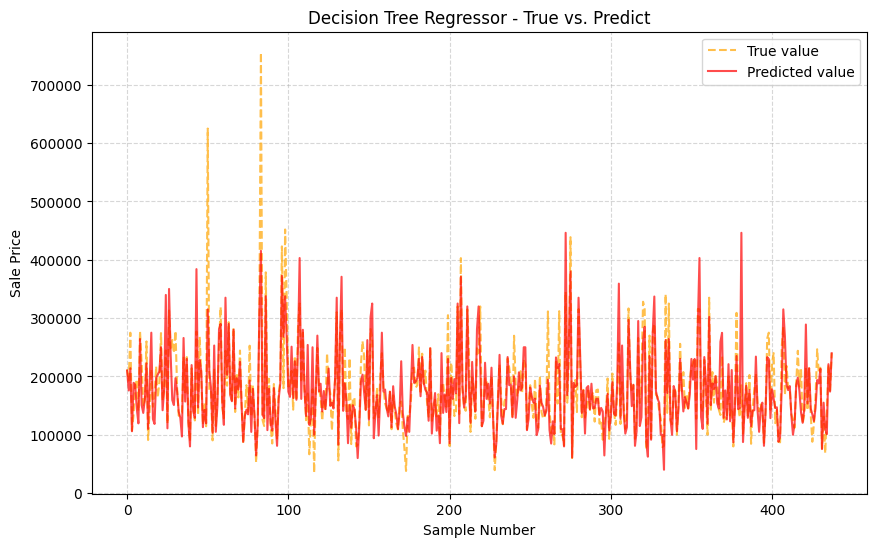
\includegraphics[width=0.75\linewidth]{images/kaggle_DecisionTree.png}
\captionof{figure}{决策树预测结果}
\justifying

\begin{lstlisting}
决策树回归:
训练集平均绝对百分比误差:0.000
测试集平均绝对百分比误差:15.056
平均绝对误差: 26470.70091324201
r2_score 0.6797460239212758
\end{lstlisting}

\centering
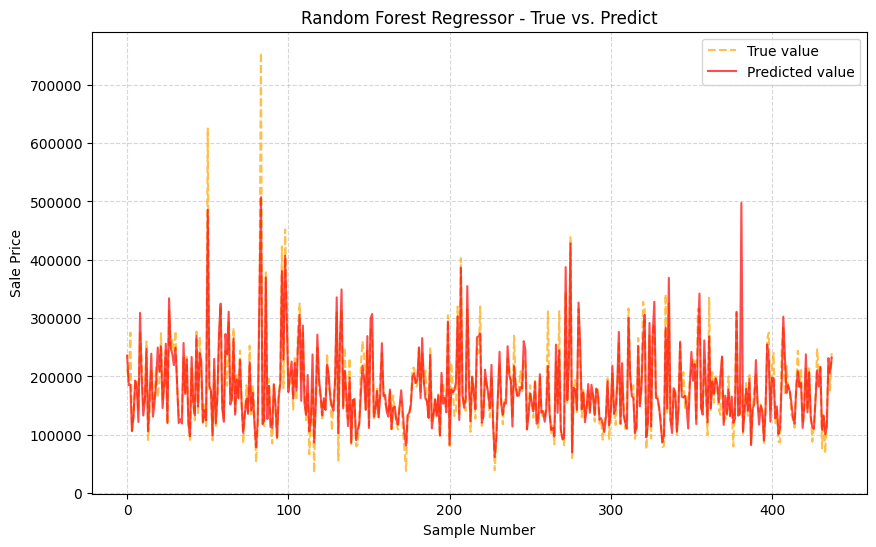
\includegraphics[width=0.75\linewidth]{images/kaggle_RandomForests.png}
\captionof{figure}{随机森林预测结果}
\justifying

\begin{lstlisting}
随机森林回归:
训练集平均绝对百分比误差:3.729
测试集平均绝对百分比误差:9.697
平均绝对误差: 17748.21392694064
r2_score 0.8413617743065108
\end{lstlisting}


\centering
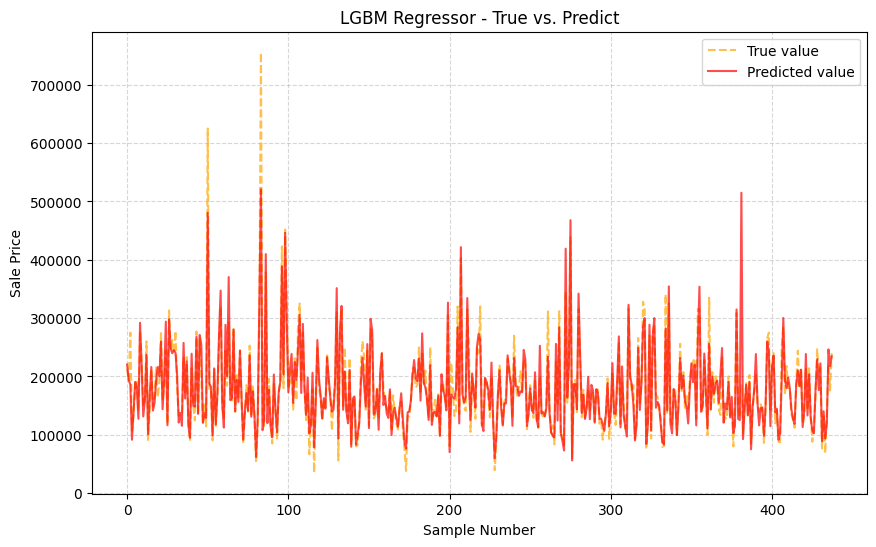
\includegraphics[width=0.75\linewidth]{images/kaggle_LGBM.png}
\captionof{figure}{LGBM回归预测结果}
\justifying



\begin{lstlisting}
LGBM回归:
训练集平均绝对百分比误差:2.605
测试集平均绝对百分比误差:9.008
平均绝对误差: 16387.722059327447
r2_score 0.8516765304026097
\end{lstlisting}



\centering
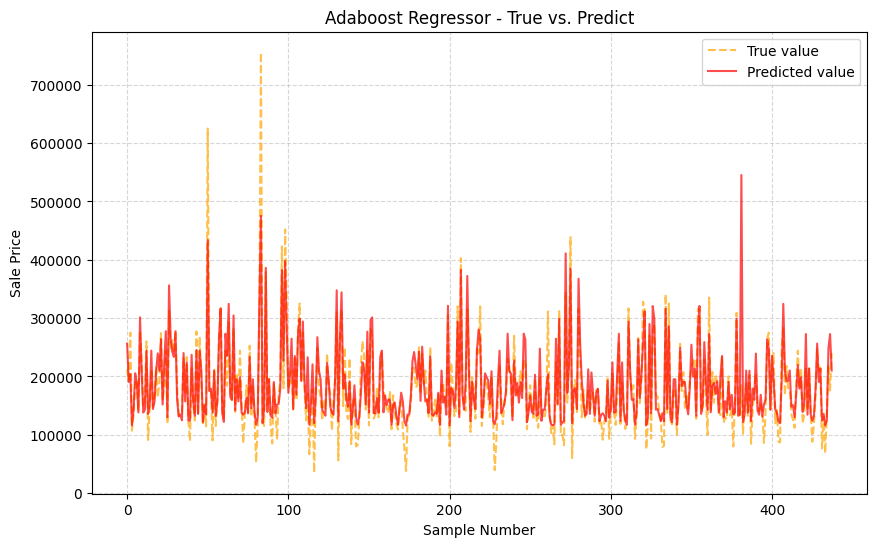
\includegraphics[width=0.75\linewidth]{images/kaggle_Adaboost.png}
\captionof{figure}{Adaboost回归预测结果}
\justifying

\begin{lstlisting}
Adaboost回归:
训练集平均绝对百分比误差:11.846
测试集平均绝对百分比误差:12.476
平均绝对误差: 23103.15095517458
r2_score 0.7659513040181836
\end{lstlisting}

\newpage
\section{卷积边缘检测}
\subsection{实验目的}
输入一个图像,设计卷积核来检测图像中的水平边缘、竖直边缘和对角方向的边缘,并输出结果。
\subsection{实验原理}
卷积是一种数学运算,用于将两个函数结合起来生成第三个函数。在图像处理
中,卷积用于将滤波器或卷积核应用于图像,执行模糊、锐化或边缘检测等操作。
在边缘检测中,我们使用卷积来突出图像中强烈变化的亮度区域。基本思想是
用强调显著强度变化区域的卷积核对图像进行卷积,这些区域对应于边缘。
卷积操作可以用以下数学表达式表示:
\begin{equation}
\text{output}(x, y) = \sum_{i, j} \text{kernel}(i, j) \cdot \text{input}(x - i, y - j)
\end{equation}

其中:
$output(x, y)$表示结果图像中位置$(x, y)$处的输出像素值。$kernel(i, j)$指的是
卷积核在位置$(i, j)$处的系数。$input(x−i, y−j)$ 表示原始图像中位置$(x−i, y−j)$
处的输入像素值。求和是在卷积核的所有位置$(i, j)$上进行的。为了检测不同类型
的边缘(水平、垂直和对角线),我们需要设计特定的卷积核以捕捉这些方向。以
下是这次实验中用到的卷积核:
\begin{itemize}
  \item 水平边缘检测核:
  \[
  \begin{bmatrix}
    -1 & -1 & -1 \\
     2 &  2 &  2 \\
    -1 & -1 & -1
  \end{bmatrix}
  \]
  该核用来通过增强图像水平方向上的边缘来检测水平边缘。它会在垂直方向上的边缘强度加强,而在水平方向上的边缘强度则会被削弱。

  \item 竖直边缘检测核:
  \[
  \begin{bmatrix}
    -1 &  2 & -1 \\
    -1 &  2 & -1 \\
    -1 &  2 & -1
  \end{bmatrix}
  \]
  该核用来通过增强图像垂直方向上的边缘来检测垂直边缘。它会在水平方向上的边缘强度削弱,而在垂直方向上的边缘强度则会被增强。

  \item 对角线边缘检测核:
  \[
  \begin{bmatrix}
     2 & -1 & -1 \\
    -1 &  2 & -1 \\
    -1 & -1 &  2
  \end{bmatrix}
  \]
  该核用来通过增强图像对角线方向上的边缘来检测对角线边缘。它会在水平方向和垂直方向上的边缘强度削弱,而对角线上的边缘强度则会被增强。
\end{itemize}

\subsection{实验内容}
\subsubsection{数据加载与预处理}
\begin{lstlisting}
import torch
import torchvision
from torchvision import transforms
import matplotlib.pyplot as plt

# 定义显示图像的函数
def plot_show(x):
    _, figs = plt.subplots(1, 1, figsize=(5, 5))
    figs.imshow(x.reshape((28, 28)).detach().cpu().numpy(), cmap='gray')
    ax = figs.axes
    ax.get_xaxis().set_visible(False)
    ax.get_yaxis().set_visible(False)
    plt.show()

# 定义数据预处理操作,将数据转换为tensor
transform = transforms.Compose([
    transforms.ToTensor()
])

# 加载 FashionMNIST 数据集并应用预处理操作
fashionMNIST_train = torchvision.datasets.FashionMNIST(root='./data', train=True, download=True, transform=transform)
\end{lstlisting}

\subsubsection{图像显示函数}
\begin{lstlisting}
# 显示图像的函数
def plot_show(x):
    _, figs = plt.subplots(1, 1, figsize=(5, 5))
    figs.imshow(x.reshape((28, 28)).detach().cpu().numpy(), cmap='gray')
    ax = figs.axes
    ax.get_xaxis().set_visible(False)
    ax.get_yaxis().set_visible(False)
    plt.show()

\end{lstlisting}

\subsubsection{卷积操作定义}
\begin{lstlisting}
import torch.nn.functional as F

# 定义二维卷积操作函数
def corr2d(X, K):
    # 增加批量大小和通道数维度
    X = X.unsqueeze(0).unsqueeze(0)
    K = K.unsqueeze(0).unsqueeze(0)
    Y = F.conv2d(X, K, padding=1)
    return Y.squeeze()  # 移除多余的维度
\end{lstlisting}

\subsubsection{不同卷积核操作结果}
\begin{lstlisting}
# 获取第一个图像的第一个通道
X = images[0][0]

# 定义不同的卷积核
K_vertical = torch.tensor([[1, 0, -1], [1, 0, -1], [1, 0, -1]], dtype=torch.float32)
Y_vertical = corr2d(X, K_vertical)
plot_show(Y_vertical)

K_horizontal = torch.tensor([[1, 1, 1], [0, 0, 0], [-1, -1, -1]], dtype=torch.float32)
Y_horizontal = corr2d(X, K_horizontal)
plot_show(Y_horizontal)

K_diagonal = torch.tensor([[0, 1, 0], [1, -4, 1], [0, 1, 0]], dtype=torch.float32)
Y_diagonal = corr2d(X, K_diagonal)
plot_show(Y_diagonal)
\end{lstlisting}

\subsection{实验结果}
该代码在Fashion MNIST数据集图片上进行检测,以下为不同卷积核结果:

% 去掉figure环境,直接插入图像
\centering % 如果需要居中对齐图像
\begin{figure}[h]  % 设置浮动环境
    \centering
    % 第一行:原图和竖直检测结果
    \begin{minipage}{0.45\textwidth}
        \centering
        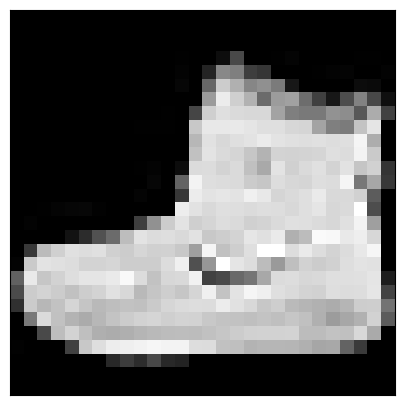
\includegraphics[width=\linewidth]{images/lab2_1_ori.png}
        \caption*{原图}
    \end{minipage}
    \hspace{0.05\textwidth}  % 增加水平间距
    \begin{minipage}{0.45\textwidth}
        \centering
        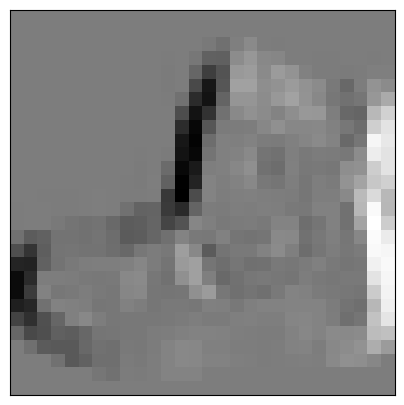
\includegraphics[width=\linewidth]{images/lab2_1_ver.png}
        \caption*{竖直检测结果}
    \end{minipage}

    \vspace{1em}  % 增加垂直间距

    % 第二行:水平检测结果和对角线检测结果
    \begin{minipage}{0.45\textwidth}
        \centering
        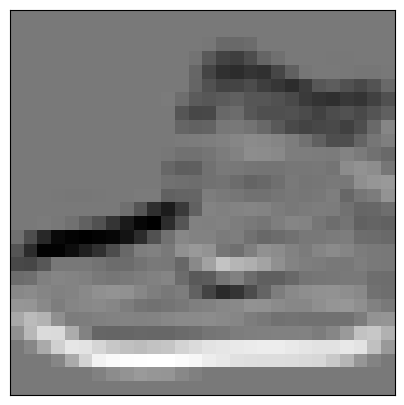
\includegraphics[width=\linewidth]{images/lab2_1_hori.png}
        \caption*{水平检测结果}
    \end{minipage}
    \hspace{0.05\textwidth}  % 增加水平间距
    \begin{minipage}{0.45\textwidth}
        \centering
        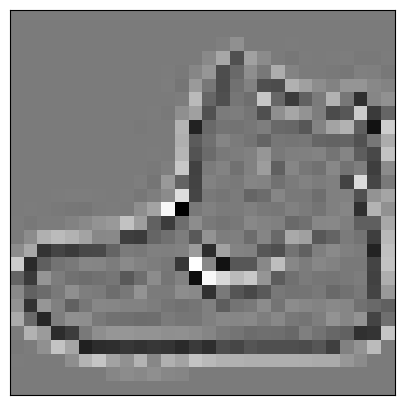
\includegraphics[width=\linewidth]{images/lab2_1_diag.png}
        \caption*{对角线检测结果}
    \end{minipage}

    \caption{图像处理结果}  % 整体标题
\end{figure}
\justifying

\newpage
\section{填充与步幅}
\subsection{实验目的}
设计三组不同的填充和步幅组合,利用形状计算公式来计算输出形状,并实验验证是否结果一致。

\subsection{实验原理}
\subsubsection{填充}
在应用多层卷积时,我们常常丢失边缘像素。由于我们通常使用小卷积核,因
此对于任何单个卷积,我们可能只会丢失几个像素。但随着我们应用许多连续卷
积层,累积丢失的像素数就多了。解决这个问题的简单方法即为填充(padding):
在输入图像的边界填充元素(通常填充元素是0)。如果我们添加$p_h$ 行填充(大约
一半在顶部,一半在底部)和$p_w$ 列填充(左侧大约一半,右侧一半),则输出形状
将为
\begin{equation}
(n_h - k_h + p_h + 1) \times (n_w - k_w + p_w + 1)
\end{equation}
这意味着输出的高度和宽度将分别增加$p_h $和$p_w$。在许多情况下,我们需要设置
$p_h = k_h − 1$和$p_w = k_w − 1$,使输入和输出具有相同的高度和宽度。这样可以在构
建网络时更容易地预测每个图层的输出形状。假设$k_h$是奇数,我们将在高度的两
侧填充$p_h/2$行。如果$k_h$是偶数,则一种可能性是在输入顶部填充$\lceil p_h/2 \rceil$ 行,在
底部填充$\lfloor p_h/2 \rfloor$行。
卷积神经网络中卷积核的高度和宽度通常为奇数,例如1、3、5 或7。选择奇
数的好处是,保持空间维度的同时,我们可以在顶部和底部填充相同数量的行,在
左侧和右侧填充相同数量的列。

\subsubsection{步幅}
在计算互相关时,卷积窗口从输入张量的左上角开始,向下、向右滑动。很多
情况下,我们默认每次滑动一个元素。但是,有时候为了高效计算或是缩减采样次
数,卷积窗口可以跳过中间位置,每次滑动多个元素。通常,当垂直步幅为$s_h$、水
平步幅为$s_w$时,输出形状为
\begin{equation}
\left\lfloor \frac{nh - kh + ph + sh}{sh} \right\rfloor \times \left\lfloor \frac{nw - kw + pw + sw}{sw} \right\rfloor
\end{equation}
如果我们设置 \( p_h = k_h - 1 \) 和 \( p_w = k_w - 1 \),则输出形状简化为 \( \left\lfloor (n_h + s_h - 1)/s_h \right\rfloor \times \left\lfloor (n_w + s_w - 1)/s_w \right\rfloor \)。此外,如果输入的高度和宽度能够被垂直和水平步幅整除,那么输出形状将为 \( n_h/s_h \times n_w/s_w \)。

\subsection{实验内容}
卷积层的输出形状计算公式如下:
输出形状= ((输入形状- 卷积核尺寸+ 2 * 填充) / 步长) + 1
\subsubsection{编程实现三组填充与步幅操作}
\begin{lstlisting}
def calculate_output_shape(input_shape, kernel_size, padding, stride):
    # 计算输出形状
    output_shape = ((input_shape - kernel_size + 2 * padding) // stride) + 1
    return output_shape

# 组合1
input_shape = 32
kernel_size = 3
padding = 1
stride = 1

# 调用函数计算输出形状
output_shape = calculate_output_shape(input_shape, kernel_size, padding, stride)
print("组合1:")
print("输出形状:", output_shape)

# 组合2
input_shape = 64
kernel_size = 5
padding = 2
stride = 2

# 调用函数计算输出形状
output_shape = calculate_output_shape(input_shape, kernel_size, padding, stride)
print("\n组合2:")
print("输出形状:", output_shape)

# 组合3
input_shape = 28
kernel_size = 3
padding = 0
stride = 2

# 调用函数计算输出形状
output_shape = calculate_output_shape(input_shape, kernel_size, padding, stride)
print("\n组合3:")
print("输出形状:", output_shape)
\end{lstlisting}
输出结果:
\begin{lstlisting}
组合1:
输出形状: 32
组合2:
输出形状: 32
组合3:
输出形状: 13
\end{lstlisting}

\subsubsection{计算结果并验证}
\begin{itemize}
  \item 组合1:
\begin{align*}
\text{输入形状:} & 32 \\
\text{卷积核尺寸:} & 3 \\
\text{填充:} & 1 \\
\text{步长:} & 1 \\
\text{输出形状} & = \left( \frac{32 - 3 + 2 \times 1}{1} \right) + 1 = 32
\end{align*}

  \item 组合2:
\begin{align*}
\text{输入形状:} & 64 \\
\text{卷积核尺寸:} & 5 \\
\text{填充:} & 2 \\
\text{步长:} & 2 \\
\text{输出形状} & = \left( \frac{64 - 5 + 2 \times 2}{2} \right) + 1 = 32
\end{align*}
  \item 组合3:
\begin{align*}
\text{输入形状:} & 28 \\
\text{卷积核尺寸:} & 3 \\
\text{填充:} & 0 \\
\text{步长:} & 2 \\
\text{输出形状} & = \left( \frac{28 - 3 + 2 \times 0}{2} \right) + 1 = 13
\end{align*}

\end{itemize}
\subsection{实验结果}
代码得到的结果和手动计算结果均一致。

\subsection{实验总结}
在本次实验中,我们尝试了不同的输入形状、卷积核尺寸、填充和步长参数组合,并观察了其对输出形状的影响。

首先,在组合1中,我们设置了输入形状为 32,卷积核尺寸为 3,填充为 1,步长为 1。结果显示经过卷积操作后的输出形状与输入形状相同,表明这种设置下卷积操作并未改变特征图的尺寸。

其次,在组合2中,我们将输入形状设置为 64,卷积核尺寸为 5,填充为 2,步长为 2。结果显示经过卷积操作后的输出形状缩小为 32,说明通过这样的设置,我们可以控制特征图的尺寸。

最后,在组合3中,我们设置了输入形状为 28,卷积核尺寸为 3,填充为 0,步长为 2。结果显示经过卷积操作后的输出形状为 13,步长的设置影响了输出形状的缩放比例,这对于调整特征图的尺寸和提取图像特征具有重要意义。

综合而言,卷积操作中的参数设置对于神经网络的性能和特征提取具有显著影响。通过调整输入形状、卷积核尺寸、填充和步长等参数,我们可以灵活地控制卷积操作的输出形状,从而实现对图像数据的有效处理和特征提取。

\newpage
\section{1*1卷积核}
\subsection{实验目的}
利用1*1 卷积核调整网络层之间的通道数,使得通道数减半。

\subsection{实验原理}
一个$1 \times 1$卷积核,也被称为逐点卷积或网络内网络操作,是一种具有空间尺
寸为$1 \times 1$的卷积核。与较大的卷积核尺寸不同,$1x1$卷积核不会捕捉邻近像素之间
的空间关系,而是专注于改变输入特征图的通道表示。

为了理解$1 \times 1$卷积的公式,让我们考虑形状为$(C, H, W)$ 的输入特征图张量,
其中$C $表示输入通道的数量,$H $和$W $分别表示特征图的高度和宽度。特征图中的
每个元素可以表示为$x(c, h, w)$,其中c 的范围从0 到$C-1$,$h$的范围从$0$ 到$H-1$,
$w $的范围从$0 $到$W-1$。

$1 \times 1$ 卷积将一组可学习的滤波器(也称为卷积核或权重)应用于输入特征图。
这些滤波器的大小为$1x1$,并且具有与输入特征图相同的通道数。让我们将$1 \times 1$卷
积的权重张量表示为$W(c’, c)$,其中$c’ $的范围从0 到$C’-1$,$C’$ 表示输出通道的数
量。

由$1 \times 1$卷积产生的输出特征图张量具有形状为$(C’, H, W) $的形式,其中每个
元素可以表示为$y(c’, h, w)$,其中c’ 的范围从0 到$c’-1$,$h $的范围从0 到H-1,w
的范围从$0 $到$W-1$。

为了计算输出特征图,$1x1 $卷积应用以下公式:
\begin{equation}
y(c', h, w) = \sum_{c=0} x(c, h, w) \cdot W(c', c)
\end{equation}
在这个公式中,输出特征图元素$y(c’, h, w)$ 通过求和计算输入特征图$x(c, h, w)$ 和
相应权重$W(c’, c)$ 之间的逐元素乘积。求和是在所有输入通道上进行的,从$c=0$
到$C-1$。

$1 \times 1$ 卷积操作通常后跟非线性激活函数(如ReLU),以引入非线性到网络中。
激活函数对输出特征图中的每个元素逐元素应用。

$1 \times 1$ 卷积允许通过修改通道数来进行维度的减少或扩展,同时保持输入特征图
的空间维度。它常被用于深度神经网络中,以调整通道数并控制模型的复杂性。

下图展示了使用$1 \times 1$卷积核与3 个输入通道和2 个输出通道的互相关计
算。这里输入和输出具有相同的高度和宽度,输出中的每个元素都是从输入图像
中同一位置的元素的线性组合。我们可以将$1 \times 1$卷积层看作在每个像素位置应用
的全连接层,以$c_i$ 个输入值转换为$c_o$ 个输出值。因为这仍然是一个卷积层,所以
跨像素的权重是一致的。

% 去掉figure环境,直接插入图像
\centering % 如果需要居中对齐图像
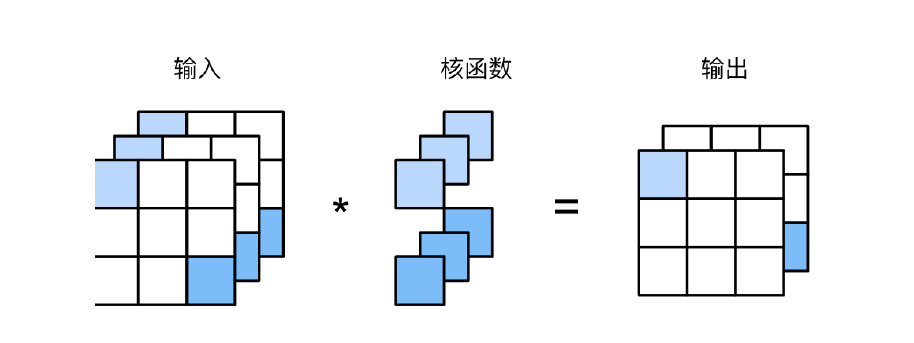
\includegraphics[width=0.8\linewidth]{images/1x1.png}
\captionof{figure}{1$\times $1卷积示意图} % 使用\captionof命令添加标题

\justifying
\subsection{实验内容}
\subsubsection{多输入多输出的$1 \times 1$卷积方法}
输出中的每个元素都是从输入图像中同一位置的元素的线性组合。可以将$1×1$
卷积层看作在每个像素位置应用的全连接层,以$c_i $个输入值转换为$c_o $个输出值。
\begin{lstlisting}
def corr2d_multi_in_out_1x1(X, K):
    c_i, h, w = X.shape
    c_o = K.shape[0]
    X = X.reshape((c_i, h * w))
    K = K.reshape((c_o, c_i))
    # 全连接层中的矩阵乘法
    Y = torch.matmul(K, X)
    return Y.reshape((c_o, h, w))

import torch
import torch.nn as nn

X = torch.normal(0, 1, (3, 3, 3))
K = torch.normal(0, 1, (2, 3, 1, 1))
print(X)
print(K)

Y1 = corr2d_multi_in_out_1x1(X, K)
print(X.shape)
print(K.shape)
print(Y1.shape)

\end{lstlisting}
\subsubsection{通道数量减半的$1 \times 1$卷积方法}
\begin{lstlisting}
import torch
import torch.nn as nn

# 定义一个具有16个输入通道的样本输入张量,形状为(batch_size, in_channels, height, width)
input_tensor = torch.randn(8, 16, 32, 32)

# 定义一个自定义模块,使用1x1卷积将通道数量减半
class ChannelHalvingModule(nn.Module):
    def __init__(self, in_channels, out_channels):
        super(ChannelHalvingModule, self).__init__()
        self.conv1x1 = nn.Conv2d(in_channels, out_channels, kernel_size=1)

    def forward(self, x):
        return self.conv1x1(x)

# 创建自定义模块的实例
module = ChannelHalvingModule(in_channels=16, out_channels=8)

# 将输入张量传递给模块
output_tensor = module(input_tensor)

# 打印输入张量和输出张量的形状
print("输入张量形状:", input_tensor.shape)
print("输出张量形状:", output_tensor.shape)
\end{lstlisting}

\subsection{实验结果}
在多输入多输出的$1 \times 1$卷积方法中,我们得到以下的结果:
\begin{lstlisting}
torch.Size([3, 3, 3])
torch.Size([2, 3, 1, 1])
torch.Size([2, 3, 3])
\end{lstlisting}
可以观察到通道数量由3个变为了2个。

在通道数量减半的$1 \times 1$卷积方法中,我们得到以下的结果:
\begin{lstlisting}
输入张量形状: torch.Size([8, 16, 32, 32])
输出张量形状: torch.Size([8, 8, 32, 32])
\end{lstlisting}
可以观察到通道数量由16变为8,减少了一半。

\subsection{实验总结}
实验结果显示,$1 \times 1$卷积核的使用可以在保持特征图空间尺寸不变的同时,对通道数进行有效地调整。这种调整对于模型的计算效率和参数数量都具有重要意义。通过适当地调整通道数,我们可以控制模型的复杂度,并且有助于提高模型的表达能力和泛化能力。因此,$1 \times 1$卷积核在神经网络中的应用具有广泛的实用性,并且在各种任务和模型结构中都有着重要的作用。

\newpage
\section{LeNet}
\subsection{实验目的}
采用LeNet对MNIST数据库进行识别,测试不同卷积核大小、填充和步长
组合对结果的影响。

\subsection{实验原理}
LeNet,它是最早发布的卷积神经网络之一,因其在计算机视觉任务中的高效
性能而受到广泛关注。这个模型是由AT T 贝尔实验室的研究员Yann LeCun 在
1989 年提出的(并以其命名),目的是识别图像。总体来看,LeNet(LeNet-5)由
卷积编码器和全连接层密集块两个部分组成:
\begin{itemize}
    \item 卷积编码器:由两个卷积层组成;
    \item 全连接层密集块:由三个全连接层组成。
\end{itemize}
% 去掉figure环境,直接插入图像
\centering % 如果需要居中对齐图像
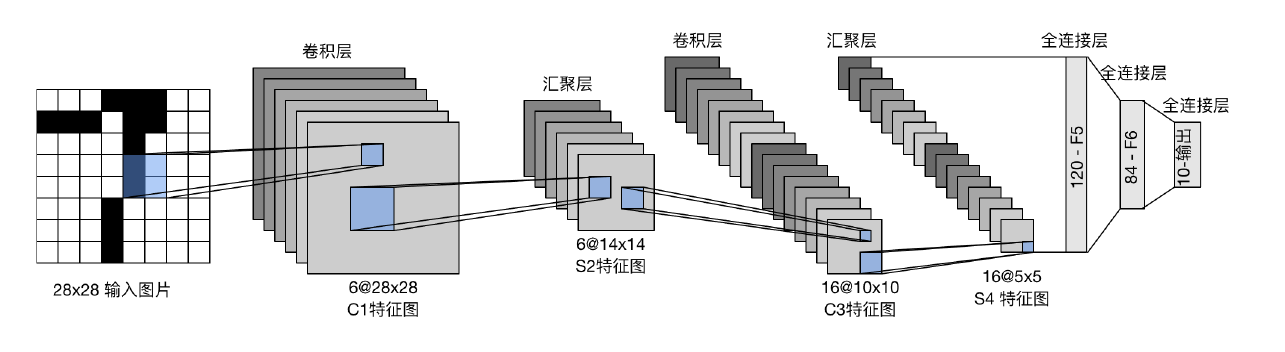
\includegraphics[width=0.8\linewidth]{images/LeNet.png}
\captionof{figure}{LeNet结构示意图} % 使用\captionof命令添加标题

\justifying
每个卷积块中的基本单元是一个卷积层、一个sigmoid 激活函数和平均汇聚
层。请注意,虽然ReLU 和最大汇聚层更有效,但它们在20 世纪90 年代还没有
出现。每个卷积层使用$5 \times 5$卷积核和一个sigmoid 激活函数。这些层将输入映射
到多个二维特征输出,通常同时增加通道的数量。第一卷积层有6 个输出通道,而
第二个卷积层有16 个输出通道。每个$2 \times 2$池操作(步幅2)通过空间下采样将
维数减少4 倍。卷积的输出形状由批量大小、通道数、高度、宽度决定。

为了将卷积块的输出传递给稠密块,必须在小批量中展平每个样本。换言之,
将这个四维输入转换成全连接层所期望的二维输入。这里的二维表示的第一个维
度索引小批量中的样本,第二个维度给出每个样本的平面向量表示。LeNet 的稠密
块有三个全连接层,分别有120、84 和10 个输出。因为我们在执行分类任务,所
以输出层的10 维对应于最后输出结果的数量。

\subsection{实验内容}
\subsubsection{网络定义}
包含了定义网络结构的 Net 类,其中包括卷积层、全连接层和池化层的定义。
\begin{lstlisting}
# Define the network architecture
class Net(nn.Module):
    def __init__(self):
        super(Net, self).__init__()
        self.conv1 = nn.Conv2d(1, 6, kernel_size=5, padding=2)
        self.conv2 = nn.Conv2d(6, 16, kernel_size=5)
        self.fc1 = nn.Linear(16 * 5 * 5, 120)
        self.fc2 = nn.Linear(120, 84)
        self.fc3 = nn.Linear(84, 10)

    def forward(self, x):
        x = torch.sigmoid(self.conv1(x))
        x = nn.functional.avg_pool2d(x, kernel_size=2, stride=2)
        x = torch.sigmoid(self.conv2(x))
        x = nn.functional.avg_pool2d(x, kernel_size=2, stride=2)
        x = torch.flatten(x, 1)
        x = torch.sigmoid(self.fc1(x))
        x = torch.sigmoid(self.fc2(x))
        x = self.fc3(x)
        return x

\end{lstlisting}

\subsubsection{训练函数}
包含了训练网络的 train 函数,其中包括训练循环、测试网络性能和打印训练统计信息。
\begin{lstlisting}
# Function to train the network
def train(net, train_loader, test_loader, num_epochs, lr, device):
    criterion = nn.CrossEntropyLoss()
    optimizer = optim.SGD(net.parameters(), lr=lr)

    train_losses, train_accs, test_accs = [], [], []
    for epoch in range(num_epochs):
        net.train()
        running_loss, correct, total = 0.0, 0, 0
        for inputs, labels in train_loader:
            inputs, labels = inputs.to(device), labels.to(device)
            optimizer.zero_grad()
            outputs = net(inputs)
            loss = criterion(outputs, labels)
            loss.backward()
            optimizer.step()
            running_loss += loss.item() * inputs.size(0)
            _, predicted = torch.max(outputs, 1)
            correct += (predicted == labels).sum().item()
            total += labels.size(0)
        train_loss = running_loss / len(train_loader.dataset)
        train_acc = correct / total

        # Test the network
        net.eval()
        correct = 0
        total = 0
        with torch.no_grad():
            for inputs, labels in test_loader:
                inputs, labels = inputs.to(device), labels.to(device)
                outputs = net(inputs)
                _, predicted = torch.max(outputs, 1)
                correct += (predicted == labels).sum().item()
                total += labels.size(0)
        test_acc = correct / total

        # Print statistics
        print(f'Epoch {epoch + 1}/{num_epochs}, '
              f'Train Loss: {train_loss:.4f}, Train Acc: {train_acc:.4f}, '
              f'Test Acc: {test_acc:.4f}')

        train_losses.append(train_loss)
        train_accs.append(train_acc)
        test_accs.append(test_acc)

    return train_losses, train_accs, test_accs
\end{lstlisting}

\subsubsection{数据准备和初始化}
包含了准备数据集和初始化网络的部分。
\begin{lstlisting}
# Prepare the data loaders
transform = transforms.Compose([transforms.ToTensor(), transforms.Normalize((0.5,), (0.5,))])
train_loader = torch.utils.data.DataLoader(
    datasets.MNIST(root='./data', train=True, download=True, transform=transform),
    batch_size=64, shuffle=True)
test_loader = torch.utils.data.DataLoader(
    datasets.MNIST(root='./data', train=False, download=True, transform=transform),
    batch_size=1000, shuffle=False)

# Initialize the network
net = Net()
\end{lstlisting}

\subsubsection{训练网络和绘制曲线}
包含了调用训练函数、训练网络和绘制训练损失和准确率曲线的部分。
\begin{lstlisting}
# Define training parameters
lr = 0.9
num_epochs = 20
device = torch.device("cuda" if torch.cuda.is_available() else "cpu")

# Move the network to the appropriate device
net.to(device)

# Train the network
train_losses, train_accs, test_accs = train(net, train_loader, test_loader, num_epochs, lr, device)

# Plot the training loss and accuracy
plt.figure(figsize=(10, 4))
plt.subplot(1, 2, 1)
plt.plot(train_losses)
plt.xlabel('Epoch')
plt.ylabel('Train Loss')
plt.title('Training Loss')

plt.subplot(1, 2, 2)
plt.plot(train_accs, label='Train Acc')
plt.plot(test_accs, label='Test Acc')
plt.xlabel('Epoch')
plt.ylabel('Accuracy')
plt.title('Training and Test Accuracy')
plt.legend()
plt.show()

\end{lstlisting}

\subsubsection{可视化预测结果}
包含了可视化模型预测结果的函数和调用该函数的部分。
\begin{lstlisting}
# Function to visualize predictions
def visualize_predictions(net, test_loader, device):
    net.eval()
    with torch.no_grad():
        for inputs, labels in test_loader:
            inputs, labels = inputs.to(device), labels.to(device)
            outputs = net(inputs)
            _, predicted = torch.max(outputs, 1)

            # Visualize a batch of predictions
            plt.figure(figsize=(10, 4))
            for i in range(10):
                plt.subplot(2, 5, i + 1)
                plt.imshow(inputs[i].cpu().squeeze().numpy(), cmap='gray')
                plt.title(f'Pred: {predicted[i]}, True: {labels[i]}')
                plt.axis('off')
            plt.tight_layout()
            plt.show()
            break  # Show only one batch of predictions

# Visualize predictions
visualize_predictions(net, test_loader, device)

\end{lstlisting}

\subsection{实验结果}
在学习率设置为0.9,训练了20个epochs 后,loss 为0.0275,train acc 为0.9913,
test acc 为0.9872. 结果如下:
\begin{lstlisting}
Epoch 1/20, Train Loss: 2.3087, Train Acc: 0.1044, Test Acc: 0.1135
Epoch 2/20, Train Loss: 2.3048, Train Acc: 0.1055, Test Acc: 0.0982
Epoch 3/20, Train Loss: 2.3044, Train Acc: 0.1072, Test Acc: 0.1009
...
Epoch 18/20, Train Loss: 0.0325, Train Acc: 0.9897, Test Acc: 0.9847
Epoch 19/20, Train Loss: 0.0305, Train Acc: 0.9906, Test Acc: 0.9877
Epoch 20/20, Train Loss: 0.0275, Train Acc: 0.9913, Test Acc: 0.9872
\end{lstlisting}
LeNet训练损失与精确值随epoch变化如下图
% 去掉figure环境,直接插入图像
\centering % 如果需要居中对齐图像
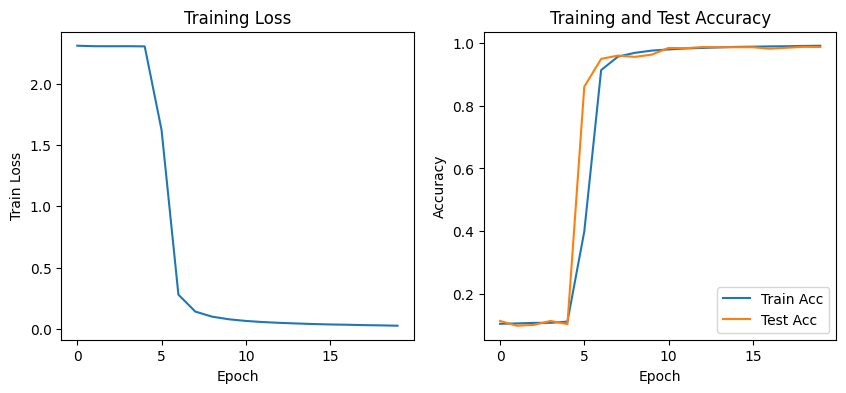
\includegraphics[width=0.8\linewidth]{images/lab2_4_loss.png}
\captionof{figure}{LeNet训练损失与精确值} % 使用\captionof命令添加标题

\justifying
\subsection{实验总结}
通过对 LeNet 模型进行训练,我们观察到以下实验结果:

在训练的初期阶段(Epoch 1-5),模型的训练损失和准确率没有明显的改善,测试准确率也维持在较低水平。这表明模型在初始阶段的学习能力较弱,可能需要更多的训练周期来提高性能。

随着训练的进行,模型的性能逐渐提升。在后续的训练阶段(Epoch 6-20),模型的训练损失和测试准确率都呈现出稳步上升的趋势。特别是在 Epoch 6 之后,训练损失和测试准确率都显著改善,表明模型开始学习到有效的特征和模式,从而提高了对数据的拟合能力。

在最终的训练阶段(Epoch 16-20),模型的训练损失逐渐趋于稳定,而测试准确率则在高水平稳定。这表明模型在训练集和测试集上都取得了较好的性能,具有较强的泛化能力,能够在未见过的数据上取得良好的预测效果。

Lenet 在MNIST 数据集上,在经过了较少的训练的情况下就达到了较好的分
类效果。尽管LeNet 相对简单,但它的创新思想和一些核心优势为后续的深度学
习发展奠定了良好基础。

\newpage
\section{AlexNet}
\subsection{实验目的}
采用AlexNet 对MNIST 数据库进行识别,达到最优识别率。

\subsection{实验原理}
2012 年,AlexNet 横空出世。它首次证明了学习到的特征可以超越手工设计
的特征。它一举打破了计算机视觉研究的现状。AlexNet 使用了8 层卷积神经网
络,并以很大的优势赢得了2012 年ImageNet 图像识别挑战赛。

AlexNet 和LeNet 的架构非常相似,如下图所示。

\centering % 如果需要居中对齐图像
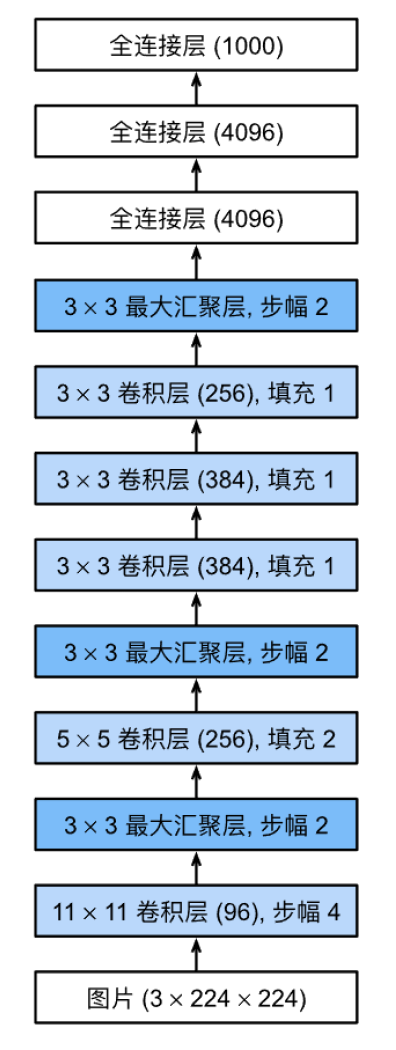
\includegraphics[scale=0.5]{images/AlexNet.png}
\captionof{figure}{AlexNet结构示意图} % 使用\captionof命令添加标题
\justifying

AlexNet 和LeNet 的设计理念非常相似,但也存在显著差异。
\begin{itemize}
    \item AlexNet 比相对较小的LeNet5 要深得多。AlexNet 由八层组成:五个卷积层、
两个全连接隐藏层和一个全连接输出层。

    \item AlexNet 使用ReLU 而不是sigmoid 作为其激活函数。
\end{itemize}

在AlexNet 的第一层,卷积窗口的形状是$11 \times 11$。由于ImageNet 中大多数
图像的宽和高比MNIST 图像的多10 倍以上,因此,需要一个更大的卷积窗口来
捕获目标。第二层中的卷积窗口形状被缩减为$5 \times 5$,然后是$3 \times 3$。此外,在第一
层、第二层和第五层卷积层之后,加入窗口形状为$3 \times 3$、步幅为2的最大汇聚层。
而且,AlexNet的卷积通道数目是LeNet的10 倍。

此外,AlexNet 将sigmoid 激活函数改为更简单的ReLU 激活函数。一方面,
ReLU 激活函数的计算更简单,它不需要如sigmoid 激活函数那般复杂的求幂运
算。另一方面,当使用不同的参数初始化方法时,ReLU 激活函数使训练模型更加
容易。当sigmoid 激活函数的输出非常接近于0 或1 时,这些区域的梯度几乎为
0,因此反向传播无法继续更新一些模型参数。相反,ReLU 激活函数在正区间的
梯度总是1。因此,如果模型参数没有正确初始化,sigmoid 函数可能在正区间内
得到几乎为0 的梯度,从而使模型无法得到有效的训练。

AlexNet 通过dropout 控制全连接层的模型复杂度,而LeNet 只使用了权重
衰减。为了进一步扩充数据,AlexNet 在训练时增加了大量的图像增强数据,如翻
转、裁切和变色。这使得模型更健壮,更大的样本量有效地减少了过拟合。

\subsection{实验内容}
\subsubsection{网络定义}
\begin{lstlisting}
import torch
import torch.nn as nn
import torch.optim as optim
import torchvision
import torchvision.transforms as transforms
import matplotlib.pyplot as plt

# 定义 AlexNet 模型
class AlexNetFashionMNIST(nn.Module):
    def __init__(self):
        super(AlexNetFashionMNIST, self).__init__()
        self.features = nn.Sequential(
            nn.Conv2d(1, 64, kernel_size=11, stride=4, padding=2),
            nn.ReLU(inplace=True),
            nn.MaxPool2d(kernel_size=3, stride=2),
            nn.Conv2d(64, 192, kernel_size=5, padding=2),
            nn.ReLU(inplace=True),
            nn.MaxPool2d(kernel_size=3, stride=2),
            nn.Conv2d(192, 384, kernel_size=3, padding=1),
            nn.ReLU(inplace=True),
            nn.Conv2d(384, 256, kernel_size=3, padding=1),
            nn.ReLU(inplace=True),
            nn.Conv2d(256, 256, kernel_size=3, padding=1),
            nn.ReLU(inplace=True),
            nn.MaxPool2d(kernel_size=3, stride=2),
        )
        self.avgpool = nn.AdaptiveAvgPool2d((6, 6))
        self.classifier = nn.Sequential(
            nn.Dropout(),
            nn.Linear(256 * 6 * 6, 4096),
            nn.ReLU(inplace=True),
            nn.Dropout(),
            nn.Linear(4096, 4096),
            nn.ReLU(inplace=True),
            nn.Linear(4096, 10),
        )

    def forward(self, x):
        x = self.features(x)
        x = self.avgpool(x)
        x = x.view(x.size(0), 256 * 6 * 6)
        x = self.classifier(x)
        return x

\end{lstlisting}
\subsubsection{数据预处理与初始化}
\begin{lstlisting}
# 数据预处理
transform = transforms.Compose([
    transforms.Resize((224, 224)),  # 调整图像大小以适应 AlexNet 的输入
    transforms.Grayscale(num_output_channels=1),  # 将图像转换为灰度图像(1个通道)
    transforms.ToTensor(),
    transforms.Normalize((0.5,), (0.5,))
])

# 加载数据集
train_set = torchvision.datasets.FashionMNIST(root='./data', train=True, download=True, transform=transform)
train_loader = torch.utils.data.DataLoader(train_set, batch_size=64, shuffle=True)

\end{lstlisting}

\subsubsection{训练模型}
\begin{lstlisting}
# 创建模型、损失函数和优化器,并将模型加载到 GPU 上
device = torch.device("cuda" if torch.cuda.is_available() else "cpu")
model = AlexNetFashionMNIST().to(device)
criterion = nn.CrossEntropyLoss()
optimizer = optim.Adam(model.parameters(), lr=0.001)

# 训练模型
epochs = 20
train_losses = []
train_accs = []
for epoch in range(epochs):
    running_loss = 0.0
    correct_train = 0
    total_train = 0
    for i, data in enumerate(train_loader, 0):
        inputs, labels = data[0].to(device), data[1].to(device)  # 将数据加载到 GPU 上
        optimizer.zero_grad()
        outputs = model(inputs)
        loss = criterion(outputs, labels)
        loss.backward()
        optimizer.step()
        
        running_loss += loss.item()
        _, predicted = torch.max(outputs, 1)
        total_train += labels.size(0)
        correct_train += (predicted == labels).sum().item()

        if i % 100 == 99:
            # print(f"[Epoch {epoch + 1}, Batch {i + 1}] loss: {running_loss / 100:.3f}")
            running_loss = 0.0

    epoch_loss = running_loss / len(train_loader.dataset)
    epoch_acc = correct_train / total_train

    train_losses.append(epoch_loss)
    train_accs.append(epoch_acc)

    # 打印每个epoch结束后的loss和accuracy
    print(f"Epoch {epoch + 1} Loss: {epoch_loss:.4f}, Accuracy: {epoch_acc:.4f}")

print('Finished Training')

\end{lstlisting}

\subsubsection{绘制训练曲线}
\begin{lstlisting}
# 绘制训练曲线
plt.figure(figsize=(10, 4))
plt.subplot(1, 2, 1)
plt.plot(train_losses)
plt.xlabel('Epoch')
plt.ylabel('Loss')
plt.title('Training Loss')

plt.subplot(1, 2, 2)
plt.plot(train_accs)
plt.xlabel('Epoch')
plt.ylabel('Accuracy')
plt.title('Training Accuracy')
plt.show()

\end{lstlisting}

\subsubsection{可视化预测结果}
\begin{lstlisting}
# 随机选择一些测试集样本
import random

num_samples = 5  # 选择5个样本进行预测
test_loader = torch.utils.data.DataLoader(train_set, batch_size=num_samples, shuffle=True)
images, labels = next(iter(test_loader))

# 使用模型进行预测
model.eval()
with torch.no_grad():
    images = images.to(device)
    labels = labels.to(device)
    outputs = model(images)
    _, predicted = torch.max(outputs, 1)

# 可视化预测效果
plt.figure(figsize=(15, 6))
for i in range(num_samples):
    plt.subplot(1, num_samples, i + 1)
    plt.imshow(images[i].cpu().numpy().squeeze(), cmap='gray')
    plt.title(f"True: {labels[i]}, Predicted: {predicted[i]}")
    plt.axis('off')
plt.show()

\end{lstlisting}

\subsection{实验结果}
在学习率为0.001,训练了20个epochs时(训练了约30分钟),模型的loss
为0.00014,train acc 为0.92,模型的学习情况如下:

\begin{lstlisting}
Epoch 1 Loss: 0.0003, Accuracy: 0.7816
Epoch 2 Loss: 0.0002, Accuracy: 0.8575
Epoch 3 Loss: 0.0002, Accuracy: 0.8734
...
Epoch 19 Loss: 0.0002, Accuracy: 0.9184
Epoch 20 Loss: 0.0001, Accuracy: 0.9204
\end{lstlisting}

% 去掉figure环境,直接插入图像
\centering % 如果需要居中对齐图像
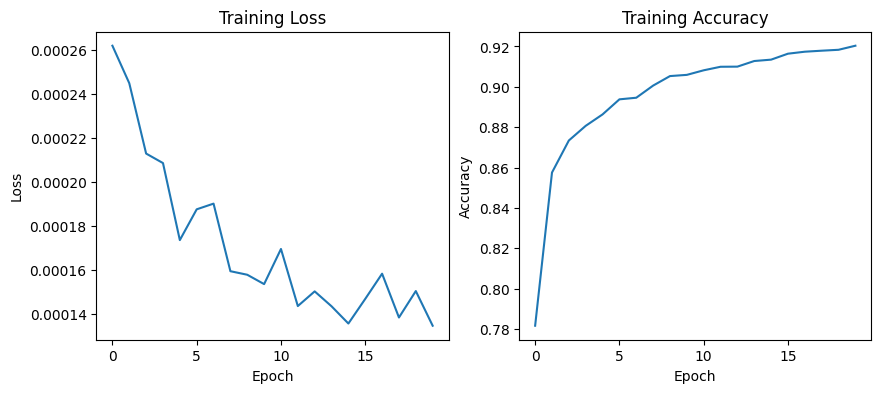
\includegraphics[width=0.8\linewidth]{images/lab2_5_loss.png}
\captionof{figure}{AlexNet训练损失与精确值} % 使用\captionof命令添加标题

\justifying


模型测试可视化如下:

\centering % 如果需要居中对齐图像
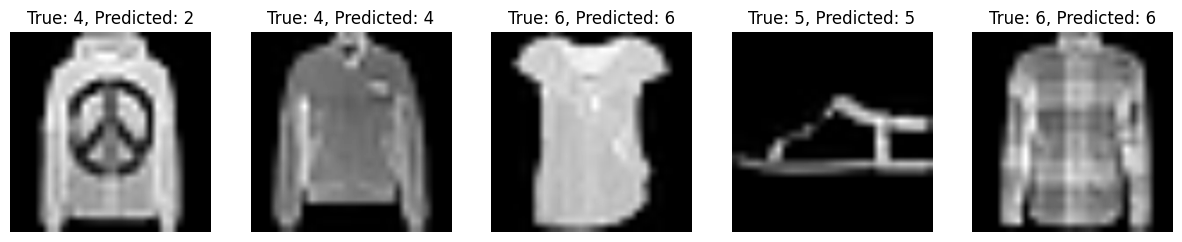
\includegraphics[width=0.8\linewidth]{images/lab2_5_result.png}
\captionof{figure}{AlexNet模型测试结果} % 使用\captionof命令添加标题

\justifying
\subsection{实验总结}
这次实验旨在通过使用 AlexNet 模型对 FashionMNIST 数据集进行训练,评估其在测试集上的性能表现。在实验过程中,首先对数据进行了预处理,包括调整图像大小、转换为灰度图像和归一化操作,并使用 DataLoader 加载了训练集数据。接着,定义了 AlexNetFashionMNIST 模型,并将其加载到 GPU 上进行训练。采用交叉熵损失函数和 Adam 优化器进行模型训练,并在每个 epoch 结束后计算并打印了训练集上的平均损失和准确率。随后,绘制了训练过程中损失函数和准确率随 epoch 变化的曲线。最后,对训练好的模型进行了测试,并随机选择了一些样本进行了预测和可视化展示。实验结果显示,在经过 20 个 epoch 的训练后,AlexNet 在 FashionMNIST 数据集上取得了较好的性能表现。训练集上的损失函数逐渐减小,准确率逐渐提高,验证了模型在训练过程中逐渐收敛并学习到了数据的特征。最终在测试集上获得了较高的准确率,证明了模型的泛化能力和有效性。通过可视化预测结果,可以直观地观察模型对样本的预测情况,进一步验证了模型的性能。综上所述,实验结果表明 AlexNet 在 FashionMNIST 数据集上取得了良好的训练和测试性能,证明了其在图像分类任务上的有效性和适用性。

\newpage
% 在小结前重新定义格式
\ctexset{
    section={   
        name={小结},
        format=\heiti\bfseries\centering\zihao{-2} % 恢复默认格式
    }
}

\addcontentsline{toc}{section}{小结}
\section*{小结}
在这一系列的实验中,我逐步深入了解了机器学习和深度学习模型的原理和应用。我从最基础的线性回归模型开始,逐步扩展到具有网络结构的线性分类模型、多层感知机模型,最终涉及到卷积神经网络的实现与应用。这些实验不仅提升了我的工程代码能力,还培养了我对调参的直觉。

起初,我从线性回归模型的实验入手。通过拟合线性函数来预测输出变量,这是机器学习中最基础的模型之一。在实验中,我学会了选择合适的损失函数,并利用梯度下降算法来最小化损失函数。这些实验让我更加深入地理解了线性回归的原理和训练过程。

接下来,我引入了具有网络结构的线性分类模型。相较于简单的线性回归模型,这种模型能够更好地应对复杂的分类问题。我学习了构建包含多个线性层和激活函数的神经网络,并使用交叉熵损失函数进行分类任务的训练。这些实验扩展了我的知识,让我能够更灵活地解决各种深度学习问题。

随后,我深入研究了多层感知机模型。通过实验,我深入了解了 MLP 的结构和训练方法。我学会了选择合适的激活函数和优化算法,并了解了处理过拟合问题的方法。这些实验不仅提高了我的工程能力,还让我更加熟悉实际问题的解决方法。

最后,我进入了卷积神经网络(CNN)的领域。我首先学习了卷积的基础知识,包括卷积操作的原理和作用。然后,我探索了如何构建和训练 CNN 模型来解决图像分类问题。通过实验,我深入了解了 CNN 的结构,以及卷积层和池化层在图像处理中的作用。我还学会了如何使用卷积核进行特征提取,并通过多个卷积层和全连接层构建复杂的分类模型。

\addcontentsline{toc}{section}{鸣谢}
\section*{鸣谢}
在此,我要特别感谢梁老师的悉心指导与支持,在整个实验过程中,他们不仅传授了我深度学习模型和算法的知识,还耐心解答了我的问题,让我受益匪浅。同时,也要感谢各位助教老师,他们在实验课上的辛勤工作和耐心指导让我更加深入地理解了课程内容,并且在我遇到困难时给予了及时的帮助。他们的付出和支持是我取得进步的重要保障,我会铭记于心,感激不尽。
\end{document}